\documentclass[11pt]{report}
\usepackage{a4wide,parskip,times, complexity, amsthm,graphicx,verbatim}
\usepackage{amsfonts}
\usepackage[ruled]{algorithm2e}
\renewcommand{\algorithmcfname}{ALGORITHM}
\SetAlFnt{\small}
\SetAlCapFnt{\small}
\SetAlCapNameFnt{\small}
\SetAlCapHSkip{0pt}
\IncMargin{-\parindent}


\newclass{\GISO}{GI}
\newclass{\CGISO}{CGI}
\newclass{\paraNP}{para-NP}
\newclass{\INDSET}{INDEPENDENT-SET}

\newtheorem{thm}{Theorem}
\newtheorem{lem}[thm]{Lemma}
\newtheorem{claim}{Claim}
\newtheorem{cor}{Corollary}
\newtheorem{defn}{Definition}
\newtheorem{conj}{Conjecture}
\newcommand{\vcn}{\mbox{\emph{VCN}}}
\newcommand{\cross}{\mbox{\emph{cross}}}
%\newcommand{\td}{\mbox{\emph{td}}}

\begin{document}
	
\thispagestyle{empty}
%\pagestyle{empty}

\centerline{\LARGE Parameterized Complexity and Graph Isomorphism}
\vspace{2em}
\centerline{\Large Adam M. Bouland, St. John's College}
\centerline{\Large MPhil in Advanced Computer Science, University of Cambridge}
\centerline{\Large Project Supervisor: Prof. Anuj Dawar}
\centerline{\Large \today}
\vspace{1em}
%\centerline{\large Project Supervisor: Prof. Anuj Dawar}
\vspace{1em}


\newpage
\thispagestyle{empty}
%\pagestyle{empty}

I, Adam Michael Bouland of St. John's College, being a candidate for the M.Phil in Advanced Computer Science, hereby declare that this report and the work described in it are my own work, unaided except as may be specified below, and that the report does not contain material that has already been used to any substantial extent for a comparable purpose.

Word count: 14,942

Signed

Date 





\begin{abstract}
\textsl{Graph Isomorphism ($\GISO$) is one of the few natural problems in $\NP$ which is not known to be either in $\P$ or $\NP$-complete. The notion of fixed-parameter tractability provides a lens through which we can explore the structure of the complexity of $\GISO$. It is unknown if Graph Isomorphism is fixed-parameter tractable for many interesting parameterizations of the problem. In this dissertation we review current knowledge of the parameterized complexity of $\GISO$. We then attempt to show that graph isomorphism is fixed-parameter tractable when parameterized by three parameters, namely max leaf number, crossing number and tree-depth. We successfully show that  $\GISO$ is fixed-parameter tractable with respect to max leaf number.  We then provide evidence that $\GISO$ parameterized by crossing number may be reducible to $\GISO$ parameterized by path-width.  Finally, we show that if a certain plausible conjecture holds, then graph isomorphism is fixed-parameter tractable with respect to tree-depth. This research has the potential to give new insights into graph isomorphism, and could aid in showing that graph isomorphism is fixed-parameter-tractable with respect to path-width in future work.} 
\end{abstract}



%\newpage
\tableofcontents
%\newpage






\chapter{Introduction}

\section{Graph Isomorphism and its Classical Complexity}

	A graph $G$ is a set of vertices $V(G)$ and a symmetric irreflexive binary relation $E(G)$ on the vertices. Given graphs $G$ and $H$,we say that $G$ and $H$ are isomorphic if there exists a bijection $f:V(G)\to V(H)$ which preserves the edge relation, that is which obeys $(x,y)\in E(G) \Leftrightarrow (f(x), f(y)) \in E(H)$.

\begin{figure}[b]
\begin{center}
\leavevmode
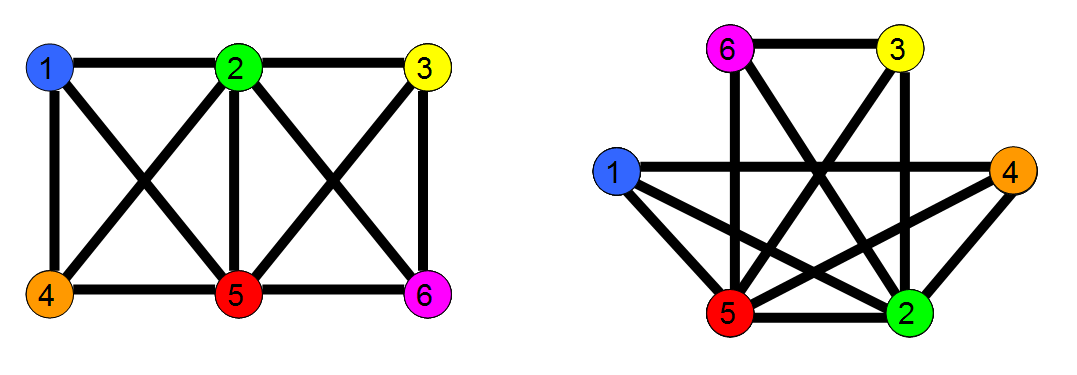
\includegraphics[height=50mm]{Graph_Isomorphism_v0.png}
\end{center}
\caption{Two isomorphic graphs. The map which preserves the labels/colours of the graphs is an isomorphism between them.}
\label{fig:one}
\end{figure}

Given graphs $G$ and $H$, the Graph Isomorphism Problem ($\GISO$) is to decide whether or not $G \cong H$. This decision problem  is clearly in $\NP$, since an isomorphism $f$ described above serves as a witness to $G\cong H$. Graph Isomorphism is not known to  have a polynomial time algorithm. Furthermore, evidence suggests that GI is not $\NP$-complete. Babai showed that the complement of $\GISO$ is in $\AM$, the set of problems decidable with probabilistic interactive proof systems \cite{Babai1985}. This impies that if $\GISO$ is $\NP$-complete, the polynomial hierarchy collapses to its second level. Since the polynomial hierarchy is not believed to collapse, this is strong evidence against the $\NP$-hardness of $\GISO$. By Ladner's theorem, we know that if $\P \neq \NP$ then there exist $\NP$-intermediate lanagues which are in $\NP$ but not $\NP$-complete \cite{Ladner75}. $\GISO$ is therefore a strong candidate to be an $\NP$-intermediate lanaguage.



\begin{figure}[h]
\begin{center}
\leavevmode
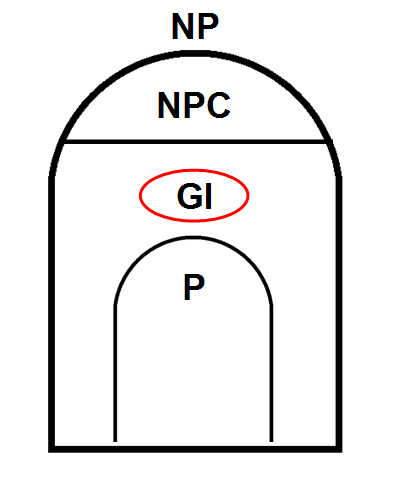
\includegraphics[height=50mm]{GI_P_NP_v0.png}
\end{center}
\caption{The location of $\GISO$ in the classical complexity hierarchy - if $\P \neq \NP$ then evidence suggests that $\GISO$ is $\NP$-intermediate.}
\label{fig:two}
\end{figure}


No polynomial time algorithm for $\GISO$ is known in the general case. The best known exact algorithm for general graphs runs in time $2^{O(\sqrt{n\llog n})}$\cite{BabaiLuks83}. 


\section{Parameterized Complexity}


Parameterized complexity studies the computational complexity of parameterizations of classical problems. Suppose we define a language $Q$ over a finite alphabet $\Sigma$ so $Q \subseteq \Sigma ^*$. $Q$ represents a classical decision problem: given $x\in \Sigma ^*$ we would like to decide whether or not $x \in Q$. Let $n=\| x \|$, the length of the input $x$. Classical complexity classifies decision problems $Q$ based on how long it takes to decide whether or not $x \in Q$ as a function of $n$. Languages which can be decided in time polynomial in $n$ are considered tractable. 
 
A parameterization of a language $Q$ is a function $\kappa : \Sigma ^* \rightarrow \mathbb{N} $ such that $\kappa$ is computable \cite{FlumGrohe}. For instance, if $G$ is a graph, we might take as the parameter the maximal degree of $G$. Given a parameterization  $\kappa$ of $Q$, we define a parameterized language to be a pair $(Q,\kappa)$. Parameterized complexity classifies parameterized decision problems  $(Q,\kappa)$ based on how long it takes to decide whether or not $x \in Q$ as a function of both $||x||$ and $\kappa(x)$ \cite{FlumGrohe}.

The notion of fixed-parameter tractability lies at the heart of parameterized complexity. A problem is said to be fixed parameter tractable (for parameter $\kappa$)  if there exists an algorithm for the problem which runs in time \[f(\kappa (x)) * n^{c}\] where  $ f  :\mathbb{N}  \rightarrow \mathbb{N} $ is computable, $n$ is the size of the input $x$ and $c$ is a constant \cite{FlumGrohe}. Note that the degree of the polynomial, $c$, must be a constant which is independent of the value of the parameter. Hence if we are promised that the value of the parameter is $k$, we have an $n^c$ algorithm to decide the problem: once the value of the parameter is controlled, the problem becomes easy.  Also, note that the function $f$ is only required to be computable: $f$ is allowed to grow very quickly and could be exponential or super-exponential. These large constants associated with large values of the parameter mean that, on a practical level, fixed-parameter algorithms are only used when the value of the parameter is small.

$\FPT$ is defined to be the set of all parameterized languages $(Q,\kappa)$ which are fixed-parameter tractable. This complexity class serves as the parameterized analogue of $\P$.  Clearly any language $Q$ in $\P$ is also in $\FPT$ under any parameterization $\kappa$. Furthermore, many problems which are not known to be in $\P$ are in $\FPT$ under certain parameterizations. $\FPT$ therefore extends the notion of classical tractability. Given intractable problems such as $\SAT$, it is interesting to identify which parameterizations of the problem place it in $\FPT$. Any parameter $\kappa$ which places $\SAT$ in $\FPT$ is in some ways ``responsible" for making $\SAT$ intractable in the general case, since controlling this parameter leads to an efficient $n^c$ algorithm for the problem. Hence discovering $\FPT$ algorithms for difficult problems can create insights into the structure of their intractability.

In classical complexity, the notion of a poly-time reduction is used to show relationships between the complexity of different problems. In parameterized complexity, the notion of a fixed parameter Karp reduction ($\FPT$-reduction) fills this role. Given two parameterized problems $(Q,\kappa)$  over $\Sigma^{*}$ and $(Q',\kappa')$  over $\Sigma'^{*}$, we say that $(Q,\kappa) \leq _{\FPT} (Q',\kappa')$, that is ``$(Q,\kappa)$ is $\FPT$ reducible to $(Q',\kappa')$", if there exists a map $f:\Sigma^{*}\rightarrow \Sigma'^{*}$ such that $x\in Q \Leftrightarrow f(x)\in Q'$, $\|f(x)\| \leq \poly(\|x\|)$, and there exists a computable $g:\mathbb{N}\rightarrow \mathbb{N}$ such that $\kappa'(f(x)) \leq g(\kappa(x))$. This is precisely the same notion as a poly-time Karp reduction, except now we also require that the value of the parameter is bounded as a computable function of the old parameter. This ensures that if $(Q,\kappa) \leq _{\FPT} (Q',\kappa')$, and $(Q',\kappa') \in \FPT$, then $(Q,\kappa) \in \FPT$. The notion of $\FPT$-reduction allows us to define hardness results in parameterized complexity theory in precisely the same way we define hardness in classical complexity \cite{FlumGrohe}.

Parameterized complexity theory involves several additional complexity classes which form the parameterized analogues of $\EXP$ and $\NP$. The class $\XP$ is the parameterized analogue of $\EXP$; the definition is similar to that of $\FPT$ except the degree of the polynomial $c$ in the runtime of the algorithm is allowed to be a function $c(\kappa(x))$ of the parameter.  The $\W$-hierarchy is an infinite family of complexity classes which form the parameterized analogues of $\NP$. 


\section{Work completed in this dissertation}

Graph Isomorphism is believed to be computationally intractable in the general case. In this project, we set out to discover which parameterizations of graph isomorphism are fixed parameter tractable. In chapter 2, we review the known $\XP$ and $\FPT$ parameterizations of graph isomorphism. Based on this review, we pick several parameterizations and try to show that $\GISO$ is in $\FPT$ under these parameterizations. In chapter 3, we show that $\GISO$ is $\FPT$ when parameterized by max leaf number and vertex cover number. In chapter 4, we explore the parameter crossing number. We create a canonical decomposition algorithm for graphs of crossing number $k$ and use this to present evidence that $(\GISO,$ crossing number$)$ may be $\FPT$-reducible to $(\GISO,$path-width$)$. Finally, in chapter 5 we show that if a certain conjecture holds then $(\GISO, $ tree-depth$)\in\FPT$. We also briefly describe how one could prove this conjecture.

Note that chapters 3 through 5 represent original mathematical work. Chapter 3 was completed in collaboration with Prof. Anuj Dawar and Dr. Matthias Mnich. Chapters 4 and 5 were developed independently under the advisorship of Prof. Anuj Dawar. 






\chapter{The status of $\GISO$ in the Parameterized Complexity Hierarchy}


This section reviews the state of knowledge of the parameterized complexity of $\GISO$. The parameterizations are listed according to their known complexity-theoretic status, and a summary of the methods used to create the most recent algorithm for each parameterization is provided. For each of the parameters listed in section \ref{sec:XP_params}, it is an open question whether or not this parameterization is in $\FPT$.


\section{Known Poly-time algorithms}


There are several classes of graphs for which polynomial-time algorithms for isomorphism testing are known. Graph Isomorphism was first shown to be in $\P$ over trees by Hopcroft and Tarjan \cite{HopcroftTarjan74}, and independently by Zemlyachenko \cite{Zemlyachenko70} \cite{Kobler2006}. This was later refined to a logspace algorithm for isomorphism testing of trees by Lindell \cite{Lindell92}. This result was further extended to show that graph isomorphism is in $\P$ over planar graphs by Hopcroft, Tarjan and Wong \cite{HopcroftTarjan72} \cite{HopcroftWong74}. The algorithm uses the fact that any 3-connected planar graph has only two possible embeddings in the plane. It then decomposes the planar graphs into 1, 2 and 3-connected components and propagates this constraint up the decomposition tree \cite{HopcroftWong74}. This algorithm was recently refined into a logspace algorithm for testing isomorphism of planar graphs by Datta et al. \cite{Datta09}.



\section{Parameterizations Known to be Fixed-Parameter Tractable}




\subsection{Size of largest colour class (coloured graph isomorphism)}

A $k$-$colouring$ of a graph $G$ is a map $f:V(G) \rightarrow \{1,2,...,k\}$. Two $k$-coloured graphs $G$ and $H$ are said to be isomorphic if there is a mapping between the vertices which preserves the edge relation as well as the colour of the vertices, i.e. a vertex of colour $i$  in $G$ must be mapped to a vertex of the same colour in $H$. The problem of deciding whether or not two coloured graphs are isomorphic is known as the Coloured Graph Isomorphism ($\CGISO$) Problem. 

Given a coloured graph $G$, the colour classes of the graph $C_i$ are taken to be the sets of vertices which share the same colour $i$, i.e. $C_i = \{v\in V(G): f(v)=i\}$. Coloured Graph Isomorphism is known to be fixed-parameter tractable when parameterized by the size of the largest colour class. This result was first shown to admit a randomized $\FPT$ algorithm by Babai \cite{Babai79}, and later was strengthened into a deterministic algorithm by Furst, Hopcroft and Luks \cite{FurstHopcroftLuks80}. It was also extended to a deterministic algorithm for coloured hypergraph isomorphism (in which the edge relation can have arity higher than two) by Arvind et al. \cite{Arvind2009}. The most general algorithm runs in time $2^{O(k)}(mn)^{O(1)}$, where $k$ is the size of the largest colour class, $n$ is the number of vertices, and $m$ is the number of hyperedges. The methods used to create these algorithms are purely algebraic, and involve the application of pointwise stabiliser series.




\subsection{Largest Multiplicity of an Eigenvalue}

Given a graph $G$, the adjacency matrix $A(G)$ is the matrix whose $(i,j)th$ entry is 1 if there is an edge from $i$ to $j$ and 0 otherwise. Graph isomorphism is fixed parameter tractable with respect to the largest multiplicity of an eigenvalue of $A(G)$. The algorithm was developed by Evdokimov and Ponomarenko and uses purely algebraic methods \cite{Evdokimov99}. Specifically, the algorithm produces a colouring on the cellular algebras of the graphs, and then uses a stabiliser series approach to find an isomorphism between the graphs, if one exists \cite{Evdokimov99}. The algorithm runs in time $k^{k^{O(1)}}n^{O(1)}$, where $k$ is the largest multiplicity of an eigenvalue of the input adjacency matrix, and $n$ is the number of vertices.




\subsection{Tree distance width and Path distance width}

Given a graph $G$, a tree distance decomposition of $G$ consists of a root node $r\in V(G)$, a tree $T$ with vertices $I$ and edge relation $F$, and a collection $\{ X_i | i \in I\}$ of subsets of $V(G)$ which obey the following conditions:

1. The $X_i$ 's form a partition of $V(G)$

2. For each $ v\in V(G)$, if $v\in X_i$ then for all other $w\in X_i$ , $dist(r, v)=dist(r, w)$, where $dist(v,w)$ is the distance from $v$ to $w$ along the shortest path between them.

3. For each $(v,w)\in E(G)$, where $v\in X_i$ and $w\in X_j$, either $i=j$ or $(i,j)\in F$.

The width of a tree distance decomposition of $G$ is given by $\displaystyle\max_{i}|X_i|$. The tree distance width of a graph $G$ is the minimum width of a tree distance decomposition of $G$. The path distance width of a graph is defined analogously, but where $T$ is a path rather than a tree.

Graph isomorphism is fixed parameter tractable when parameterized by tree distance width or path distance width. This was shown by Yamazaki et al. \cite{Yamazaki99}. Their algorithm is purely combinatorial in nature. The authors show that one can efficiently test for isomorphism between decompositions by iteratively building an isomorphism from the root of the decomposition outwards. They then leverage the fact that producing a minimal tree distance decomposition is $\FPT$ to achieve their result. Overall, their algorithm runs in time $f(k)O(n^3)$, where $n$ is the size of the graph and $k$ is the tree distance width of the graph. For rooted path distance width, the algorithm runs in time  $f(k)O(n^2)$.






\subsection{Maximum size of a simplicial component}

Graph isomorphism is poly-time reducible to chordal graph isomorphism, that is isomorphism over graphs in which every cycle of length $\geq$ 4 has a chord \cite{Uehara05}.  It is known that every chordal graph can be uniquely decomposed into simplicial components. Based on this decomposition, Toda shows that isomorphism over chordal graphs is $\FPT$ when parameterized by the maximum size of the simplicial components. This is achieved using purely algebraic methods; it is an open question whether this result can also be achieved using combinatorial methods. The algorithm runs in time $O(k!)n^{O(1)}$, where $n$ is the size of the graph and $k$ is the maximum size of the simplicial components in the chordal graph obtained from the reduction \cite{Uehara05} from $\GISO$ to chordal $\GISO$ \cite{Toda06}.





\subsection{Size of feedback vertex set}

Given a graph $G$, a set $S \subseteq V(G)$ is a feedback vertex set if removing $S$ from the graph makes it acyclic. Graph isomorphism is fixed-parameter tractable with respect to the size of the smallest feedback vertex set. The algorithm was developed by Kratsch and Schweitzer using combinatorial methods \cite{Kratsch09}. Intuitively, graphs with small feedback vertex sets are ``close" to forests, and graph isomorphism over forests can be decided in poly-time \cite{HopcroftWong74}. To test if two graphs are isomorphic, the authors first compute a miminal feedback vertex set $S$ of the first input graph. Then they observe that under isomorphism the image of $S$ must intersect every cycle of the second graph. They then create an isomorphism-preserving method of reducing size of the cycles in the second graph to be bounded by some function of the parameter. The remaining possible isomorphisms between the reduced graphs are explored by brute force search. The algorithm runs in time $f(k)O(n^2)$, where $n$ is the size of the graph and $k$ is the size of the minimum feedback vertex set \cite{Kratsch09}.










\section{Parameterizations Known to be in $\XP$}
\label{sec:XP_params}

The following parameters are $\XP$ parameterizations of $\GISO$: if the parameter is fixed, then isomorphism can be solved in poly-time, but the degree of this polynomial depends on the parameter. For each of these parameterizations, it is unknown if the parameterizations are fixed-parameter tractable.



\subsection{Tree-width and Path-width}

Given a graph $G$, a tree decomposition of $G$ is a tree $T$ with vertices $I$ and edge relation $F$ and a collection $\{ X_i | i \in I\}$ of subsets of $V(G)$ which obey the following conditions:

1. $\displaystyle\bigcup_{i=1}^{\infty}X_i = V(G)$

2. For each $(v,w)\in E(G)$, there is an $X_i$ such that $v\in X_i$ and $w \in X_i$

3. For all $i,j,k\in I$, if $j$ is on the path from $i$ to $k$ in $T$, then $X_i \cap X_k \subseteq X_j$

The width of a decomposition is the size of the largest $X_i$ minus one. The tree-width of a graph is the smallest width of a valid tree decomposition. The path-width is defined analogously, but where T is a path rather than a tree.

Graph isomorphism parameterized by tree-width is known to be in $\XP$. Bodlaender developed the proof using combinatorial methods. His algorithm creates a representation of the input graphs as partial $k$-trees in time $O(n^{k+2})$. Next, the algorithm  tests for isomorphism over partial $k$-trees using combinatorial methods involving the $k$-vertex separators of the graphs. The algorithm runs in time $O(n^{1+2^{2(k+1)}})$, where $k$ is the tree-width of the graph \cite{Bodlaender90}. 

Note that a graph of path-width $k$ has tree-width $\leq k$, since a path decomposition of width $k$ is also a tree-decomposition of width $k$. Since $\GISO$ is in $\XP$ when parameterized by tree-width, it is also in $\XP$ when parameterized by path-width.






\subsection{Genus} 

Given a graph $G$ and a surface $S$, an embedding of $G$ into $S$ is a map $\alpha$ from the vertices of $G$ to distinct points in $S$ and a mapping from each edge $(v,w)\in E(G)$ to a continuous curve $\gamma _{vw}: [0,1] \rightarrow S$ such that:

1. $\gamma _{vw}(0) = \alpha (v)$ and $\gamma _{vw}(1) =\alpha (w)$, so the curve starts at $v$ and ends at $w$

2. At most two curves intersect at any point in $S$, apart from at their endpoints.

Given a graph $G$, the genus of $G$ is the minimum genus surface into which $G$ can be embedded without any of the edges crossing one another, apart from at their endpoints. For instance, any planar graph has genus 0, since it can be embedded into the plane without crossing any edges.

Graph isomorphism is in $\XP$ when parameterized by genus. Miller showed this using topological methods. In his algorithm, first the graphs are embedded in a topological space of the appropriate genus. Next, each graph is used to create a labelling of 2-stable graphs to be compared. He then shows each 2-stable graph has a small number of embeddings, which can be used to run a brute force search of all remaining possibilities. The algorithm runs in time $n^{O(k)}$, where $n$ is the size of the graph and $k$ is the genus of the graph \cite{Miller80}. Grohe later showed that for each genus $k$ there exists an $l=f(k)$ such that the $l$-dimensional Weisfeiler-Leman algorithm solves isomorphism over graphs of genus $k$. This was achieved using methods from descriptive complexity. Grohe's algorithm runs in time $O(n^{f(k)})$ \cite{Grohe00}.






\subsection{Maximum Degree} 

The degree of a vertex $v\in V(G)$ , denoted $\Delta (v)$, is the number of edges incident to $v$. The maximum degree of a graph $G$, denoted $\Delta (G)$, is given by $\displaystyle\max_{v\in V(G)} \Delta (v)$. Graph isomorphism is known to be in $\XP$ when parameterized by maximum degree. The algorithm, developed by Luks, is purely algebraic and is a refinement of the algorithm developed to test isomorphism on graphs of bounded colour class size. The algorithm runs in time  $n^{f(k)}$, where $n$ is the size of the graph and $k$ is the maximum degree of the graph \cite{Luks82}.





\subsection{Size of the smallest excluded minor}

A graph $H$ is a minor of a graph $G$ (denoted $H\preceq G$) if $H$ can be obtained from a subgraph of $G$ by a sequence of edge contractions. (Recall that to contract an edge $(v,w)\in E(G)$ is to replace $v$ and $w$ with a single vertex $z$ which is adjacent to $\{ x \in V(G) : (v,x) \in E(G) \vee (w,x) \in E(G) \}$ ). A graph $G$ excludes a minor $H$ if $H$ is not a minor of $G$.

Graph isomorphism is known to be in $\XP$ when parameterized by the size of the smallest excluded minor. Ponomarenko first showed this result using a non-trivial algebraic algorithm \cite{Ponomarenko88}. Grohe later approached the problem through combinatorial and logical methods. He showed that for any class of graphs $C$ excluding a minor, there exists an $l$ such that the $l$-dimensional Weisfeiler-Leman algorithm (which runs in poly-time) decides $\GISO$ over $C$. To do this, he shows that $FP+C$ (fixed point logic with counting) captures $\P$ over any class of graphs with excluded minors \cite{Grohe10}. This, combined with a theorem of Otto \cite{Otto97}, imply the result. Their algorithms both run in time $n^{f(k)}$, where $n$ is the size of the graph and $k$ is the size of the smallest excluded minor \cite{Grohe10}.









\section{The way forward}

The fundamental parameterizations known to be in $\XP$ but not in $\FPT$ are tree-width, genus, maximum degree, and the size of the smallest excluded minor. To show $\GISO$ is in $\FPT$ for any of these parameterizations would represent a significant advance in the field. 

These fundamental parameters are related to a number of other parameters upon which graph isomorphism could be easier to solve. For instance, suppose that two parameterizations $\kappa _1$ and $\kappa_2$ are such that for every graph, $\kappa _1 \leq g(\kappa _2)$ for some computable function $g$. Then we know that if $\GISO$ is $\FPT$ with respect to $\kappa _1$, then it is also $\FPT$ with respect to $\kappa_2$. To see this, observe that if this the case, then isomorphism can be solved in time $f(\kappa_1)n^c$. When using $\kappa_2$ as a parameterization, by using the algorithm for $\kappa_1$ we can test for isomorphism in time $f(g(\kappa_2))n^c$, yielding a $\FPT$ algorithm.


Hence if two parameters are related by  $\kappa _1 \leq g(\kappa _2)$, then $\kappa _1$ is ``harder" to solve than $\kappa_2$, so $\kappa_1$ is a ``more general" parameter. This immediately gives a trivial $\FPT$ reduction between these two parameterizations, which we denote $(\GISO, \kappa_2 ) \leq_{\FPT} (\GISO, \kappa_1)$. Given a set of parameters, we can create a graph by connecting parameter $\kappa_1$ to $\kappa_2$ if $(\GISO, \kappa_2 ) \leq_{\FPT} (\GISO, \kappa_1)$. This graph provides a clear picture of the parameter landscape, in which the parameters at the top of the chart (that is, the root of the DAG) are the most fundamental ones. We produce such a chart in figure \ref{fig:img1} (next page).



\newpage

\begin{figure}[h]
%\begin{center}
\leavevmode
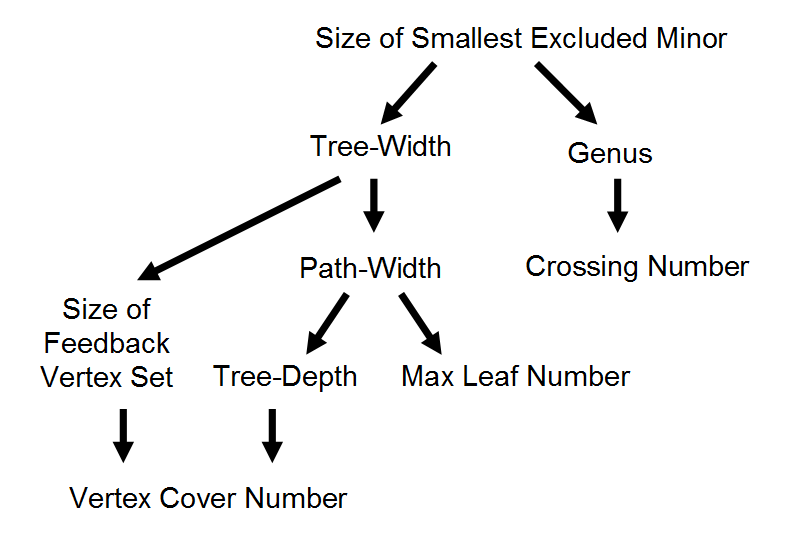
\includegraphics[height=90mm]{parameter_chart_v6.png}
%\end{center}
\caption{A chart of graph parameters. An arrow is drawn from parameter $\kappa_1$ to parameter $\kappa_2$ if $(\GISO, \kappa_2) \leq_{\FPT} (\GISO, \kappa_1)$. }
\label{fig:img1}
\end{figure}

In this dissertation, we explore the parameterizations near the bottom of the chart and attempt to show that $\GISO$ is in $\FPT$ with respect to them. We begin by showing that $\GISO$ is $\FPT$ when parameterized by max leaf number and vertex cover number. Next, we look at $\GISO$ parameterized by the crossing number. It seems plausible that graphs of low crossing number could admit a tractable algorithm, since graphs of low crossing number are ``almost planar", and $\GISO$ is in $\P$ over planar graphs. Although we do not show that $\GISO$ is $\FPT$ when parameterized by crossing number, we do present an argument that graph isomorphism parameterized by crossing number could be $\FPT$ reducible to $(\GISO,$ path-width$)$. Finally, we look at $\GISO$ when parameterized by tree-depth. By extending a tree canonization algorithm by Lindell \cite{Lindell92}, we show that if a certain plausible conjecture holds, then $\GISO$ is in $\FPT$ when parameterized by tree-depth. We leave the conjecture unproven but present techniques which we believe will allow it to be proven in the future.











\chapter{Max Leaf Number and Vertex Cover Number}

This chapter demonstrates that graph isomorphism is fixed-parameter tractable when parameterized by max leaf number and vertex cover number. Note that the vertex cover number result follows from the result for feedback vertex set, so we will only provide an outline of this proof.



\section{Max Leaf Number}

Given a connected graph $G$, a \emph{spanning tree} of $G$ is a set $F \subseteq E(G)$ such that the graph $(V(G), F)$ is a tree. A \emph{leaf } is a vertex of degree 1 in a tree. The \emph{max leaf number} of $G$ is the maximum number of leaves in a spanning tree of $G$.


\begin{figure}[h]
\begin{center}
\leavevmode
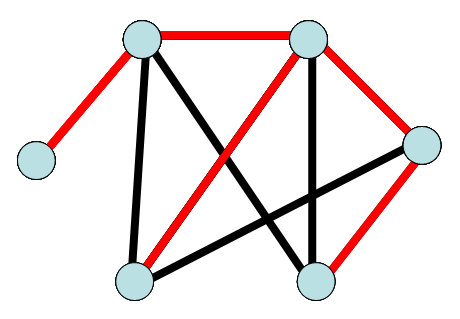
\includegraphics[height=50mm]{spanning_tree_v0.png}
\end{center}
\caption{A graph $G$, with a spanning tree of $G$ in red.}
\label{fig:spanning_tree}
\end{figure}


A graph $G$ is a subdivision of a graph $H$  if $G$ can be obtained by replacing the edges of $H$ with simple paths of length $\geq 1$. The following theorem is key to showing that graph isomorphism is fixed-parameter tractable with respect to max leaf number:

\begin{claim} Suppose $G$ is a graph with max leaf number $k$. Then $G$ is a subdivision of a graph $H$ with at most $4k-6$ vertices.
\label{mln_subdiv}
\end{claim}
\begin{proof} This theorem was cited in Fellows et al. \cite{FellowsMnich09} as a theorem from Kleitman and West \cite{KleitmanWest91}. The statement in Fellows et al. claims this holds for $4k-2$ \cite{FellowsMnich09}.

This theorem does not actually appear in Kleitman and West. However Kleitman and West do show that any graph with minimum degree 3 on $n$ vertices has a spanning tree with at least $\frac{n}{4}+2$ leaves \cite{KleitmanWest91}. They show this by creating an algorithm to construct a spanning tree of the given size on any graph of minimum degree 3. Here we work out the details omitted in \cite{FellowsMnich09} which shows that this theorem indeed follows from \cite{KleitmanWest91}.

Kleitman and West's algorithm works by greedily expanding a spanning tree $T$ with a set of operations $O1$, $O2$ and $O3$. If $G$ has maximum degree $\Delta (G)$ at least $4$, then the algorithm initializes $T$ to be all edges adjacent to a vertex of maximal degree. Otherwise, if $\Delta (G) =3$, then $T$ is initialized to be an edge which is in no triangle (If every edge of $T$ is in a triangle then T is $K_4$, which trivially has a spanning tree with the correct number of leaves).

For each vertex $x\in V(T)$, let $d'(x)$ be the number of vertices adjacent to $x$ which are not already in $T$. If $x$ is a leaf of $T$, the operation ``expand at $x$" is defined as adding all vertices adjacent to $x$ but not $T$ to the tree. If $d'(x)=0$, then $x$ is called \emph{dead}.

After initializing $T$, Kleitman and West's algorithm expands $T$ using the following operations:

$O1$: If there is a leaf $x$ of $T$ with $d'(x)\geq 2$, then expand at $x$.

$O2$: If every leaf $x$ of $T$ satisfies $d'(x)\leq 1$, and there is a leaf $x$ of $T$ adjacent to $y\notin T$ such that $y$ has at least two neighbours in $T$, then expand at $x$.


$O3$: If every leaf $x$ of $T$ satisfies $d'(x)\leq 1$ and there is no leaf $x$ whose neighbour $y$ outside of $T$ has two neighbours in $T$: Then pick an $x$ with $d'(x)=1$ adjacent to $y\notin T$ which has no other neighbours in $T$. Then expand at $x$, and subsequently expand at $y$.


If $T$ has $n$ nodes, $l$ leaves, and $m$ dead leaves ($m\leq l$), Kleitman and West show that operations $O1$ to $O3$ always satisfy the expansion inequality $3\Delta l + \Delta m \geq \Delta n $. They also show that one can always expand $T$ using one of these operations until $T$ is a spanning tree of $G$. If we expand $T$ in this manner, then summing these expansion inequalities we see that $3L + M \geq N-N_0$, where $L$ is the number of leaves in the final tree, $M$ is the number of dead leaves in the final tree, and $N_0$ is a constant related to properties of the initial spanning tree. Since $M=L$ at the end of the process, we have $4L\geq N-N_0$. Hence the graph has a spanning tree with at least $\frac{n}{4}+k_0$ leaves for some constant $k_0$. Kleitman and West show that $k_0=2$ suffices \cite{KleitmanWest91}.




To show that any graph $G$ of max leaf number $k$ is a subdivision of a graph of size at most $4k-6$, we take $G$ and create a graph $G''$ such that $G$ is a subdivision of $G''$. We then show that if $n''$ is the number of vertices in $G''$, then $G''$ has a spanning tree with $\frac{n''}{4} +2$ leaves which can be turned into a spanning tree of the same number of leaves of $G$. Hence $k\geq \frac{n''}{4} +2$, implying that $n'' \leq 4k-8$.  This holds so long as $G''$ is nonempty; in our algorithm $G''$ is empty if and only if $G$ is a path, so to handle this case we relax our constraint to $n'' \leq 4k-6$.




Consider any graph $G$ with max leaf number $k$, and create a graph $G'$ by contracting all vertices of degree 2 (that is, if a vertex $v$ of degree 2 is adjacent to $x$ and $y$, remove $v$ from the graph and add an edge from $x$ to $y$). Then G is a subdivision of $G'$. Note that $G'$ may contain self-loops, i.e. we could have $(v,v)\in E(G')$ for some $v\in V(G')$. It may also contain multiple edges between any two vertices. To correct for these, we create two gadgets as follows. Replace each self-loop from $v$ to $v$ with a cycle of length 3, i.e. create two new vertices $x$ and $y$ in $V(G'')$ such that $(v,x),(x,y),(y,v)\in E(G'')$. Replace each set of $k$ edges between vertices $v$ and $w$ with one edge from $v$ to $w$ and $k-1$ paths of length 2 from $v$ to $w$ (so we insert $k-1$ new vertices into the graph). Let $G''$ be the simple graph obtained by applying these gadgets to $G'$.



\begin{figure}[t]
\begin{center}
\leavevmode
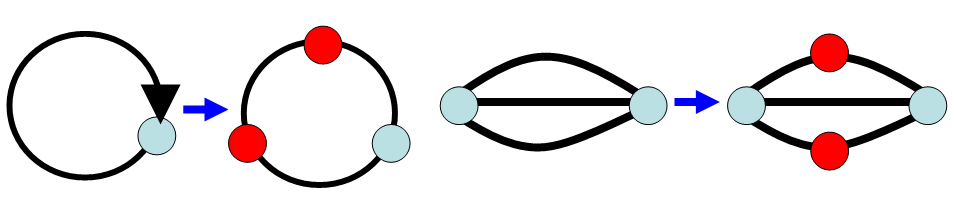
\includegraphics[height=30mm]{mln_gadgets_v0.png}
\end{center}
\caption{The gadgets used to reduce $G'$ to $G''$ in Claim \ref{mln_subdiv}. }
\end{figure}


Note that $G$ is also a subdivision of $G''$, because a self-loop in $G'$ can only be created by a path of length $\geq 3$ in $G$, and $k$ edges between two vertices in $G'$ can only be created if at least $k-1$ of them were paths of length 2 or more in $G$ . Additionally, note that the only vertices of degree 2 in $G''$ are those that we inserted using the gadgets. Furthermore, note that if $G''$ has a spanning tree with $k$ leaves, then so does $G$. 



Now run Kleitman and West's algorithm for constructing a spanning tree $T$ over $G''$. We now show that their algorithm produces a spanning tree of $G''$ with at least $\frac{n''}{4} +2$ leaves, even though $G''$ does not have minimum degree 3.  

We first take care of the vertices of degree 2 in $G''$ which were added using the reflexive edge gadget. Consider any 3-cycle $v,x,y$ added to $G''$ where $v$ is of degree $\geq 3$ and $x,y$ are of degree 2. Note that once $x$ and $y$ are added to $T$, then they are both dead so are ignored by the algorithm.

In running Kleitman and West's algorithm, if $G''$ has maximum degree $\Delta\geq 4$, then the algorithm initializes $T$ to be all edges adjacent to a vertex of maximal degree. Hence by this initialization, either $x$ and $y$ are in $T$ or neither of them are. Otherwise, $T$ is initialized to be an edge which is in no triangle (If every edge of $T$ is in a triangle then $T$ is a subdivision of $K_4$ so trivially has a spanning tree with the correct number of leaves). Since $x$ and $y$ are in a triangle, they are not in the initial $T$. Therefore either $x$ and $y$ are in $T$ initially, or neither of them are.

We now begin building the tree $T$ by operations $O1$ to $O3$. Once $v$ is added to $T$, the algorithm will immediately expand $T$ to include $x$ and $y$ using operation $O1$. From this point forward they will be dead vertices which no longer affect the algorithm. Furthermore, operation $O1$ will create changes $\Delta l = \Delta n - 1$ and $\Delta m\geq 0$, which obeys the expansion inequality. Hence $x$ and $y$ are added simultaneously to $T$ and still obey the expansion inequality. Therefore the addition of vertices of degree 2 into $G''$ as described above does not affect Kleitman and West's algorithm. 

This takes care of those vertices of degree 2 which we added using the reflexive edge gadget. Now let's take care of those vertices of degree 2 which we added using the multi-edge gadget. Let's say there were three edges from $v$ to $w$ in $G'$, and vertices $x$ and $y$ of degree 2 were added into these edges at step 1. We know that after initialization, either both $x$ and $y$ are added to $T$ or neither of them are, since they are both adjacent to the same vertices and both are part of a triangle. Additionally, they must both be added to $T$  in one operation $O1$, and afterwards are ignored by the algorithm as they are dead vertices. So this case is precisely analogous to the previous case.






We've now taken care of the vertices of degree 2 in $G''$; we now simply need to take care of the vertices of degree 1.

Consider a vertex $z$ of degree 1 in $G''$. Then $z$ is adjacent to some $v$ of degree $\geq 3$ (otherwise $G$ is a path and the theorem is trivial). Once $z$ is added to $T$, it becomes a dead leaf which is irrelevant to the algorithm. So we simply need to show that the presence of a vertex of degree $1$ does not cause any of the operations $O1$ to $O3$ to violate the expansion inequality. We showed that operation $O1$ obeys the expansion inequality regardless of the degree of the vertices to which it is expanding. The same holds for $O2$, since $O2$ results in $\Delta n =1$, $\Delta m \geq 1$ and $\Delta l =0$. So we only need to worry about operation $O3$. 

Operation $O3$ is only performed when $d'(x)\leq 1$ for every current leaf $x$ and for each leaf $x$ adjacent to $y\notin T$, $x$ is $y$'s only neighbour in $T$. Now we need to consider what happens if $y$ has degree 1. In this case $y=z$, $x=v$ has already been added to $T$, $z$ is the only neighbour of $v$ not in $T$. But now simply expanding at $v=x$, we have $\Delta n =1$, $\Delta m = 1$ (since $z$ becomes a dead vertex), and $\Delta l = 0$. This operation still obeys the expansion inequality, so by modifying $O3$ in this way in the case of a vertex of degree 1 we can preserve the expansion inequality.

This takes care of all vertices degree 1 or 2 in $G''$, thus finishing our proof.

\end{proof}

With this in hand, we can now prove a key corollary:

\begin{cor} If $G$ is a graph with max leaf number $k$, then at most $4k-6$ vertices have degree greater than or equal to three. 
\label{cor_mln_vxs}
\end{cor}
\begin{proof}
By Claim \ref{mln_subdiv} we know that $G$ is a subdivision of a graph $G'$ of size $\leq 4k-6$. Therefore $\forall v \in V(G)-V(G')$, $\Delta(v)=2$. Hence only those vertices in $V(G')$ can have degree greater than 2, so $|\{ v\in V(G): \Delta(v) \geq 3  \}| \leq |V(G')| \leq 4k-6$
\end{proof}

Suppose two graphs $G_1$ and $G_2$ are isomorphic by some isomorphism $f$. Since $f$ preserves the edge relation, $f$ preserves the degree of the vertices, so $f$ must map those vertices in $G_1$ of degree $\geq3$ to the vertices of degree $\geq3$ in $G_2$. This forms the basis for an efficient algorithm for $\GISO$ parameterized by max leaf number. The idea of the algorithm is to brute force search through all possible partial isomorphisms between the sets of vertices in each graph of degree $\geq3$. By Corollary \ref{cor_mln_vxs} this can be done in $\FPT$ time. We then test whether or not we can extend each of these partial isomorphisms between the vertices of high degree to a full isomorphism between the graphs. We know that $G_1\cong G_2$ if and only if at least one of these partial isomorphisms can be extended to a full isomorphism between the graphs. Hence this algorithm will correctly decide isomorphism between the graphs.

To turn this into a tractable algorithm for isomorphism, we need to show that testing whether these partial isomorphisms  are extendible to the whole graph is ``easy" to test. Fortunately this is the case, as the following claim demonstrates.


\begin{claim} Suppose you are given connected graphs $G_1$ and $G_2$ and nonempty sets $S=\{v\in V(G_1): \Delta(v)\geq3\}$ and $T=\{w\in V(G_1): \Delta(w)\geq3\}$ and a partial isomorphism $f:S \rightarrow T$ between $S$ and $T$.

Then, one can decide whether or not there exists an isomorphism $g:G_1 \rightarrow G_2$ which extends $f$ in time $O(n^2)$.
\label{mln_extend_iso_n2}
\end{claim}
\begin{proof}

We know that all vertices in $V(G_1)-S$ and $V(G_2)-T$ have degree less than or equal to 2. 

Consider the weighted multigraph $G_1'$ obtained from $G_1$ by replacing all simple paths in $G_1$ of length $l$ by a single edge of weight $l$. (Here a simple path means a path of vertices of degree 2). The multigraph $G_1'$ could have multiple edges between the same vertices, and could also have reflexive edges from a vertex to itself. Note that $G_1'$ is connected because $G_1$ is connected. 

Now $S \subseteq V(G_1')$, since all vertices in $S$ have degree $\geq3$ so are not part of any simple paths. Additionally, there are no vertices in $G_1'$ of degree two, since a vertex has degree two if and only if it is lies on a simple path. Hence $V(G_1') = S \cup \{v\in V(G) : \Delta(v)=1\}$.

Now modify $G_1'$ further by colouring each vertex in $v \in S$ by the multiset $\{\{ weight(e) : e=(v,w)$ for w$\in V(G_1')$ of degree 1  $\}\}$, and then removing all vertices of degree 1. Here $weight(e)$ denotes the weight of the edge $e$ in $G_1'$. Call this graph $G_1''$. 

Now $G_1''$ is a weighted connected coloured multigraph, and $V(G_1'')=S$. Construct $G_2''$ analogously. 

\begin{figure}[b!]
\begin{center}
\leavevmode
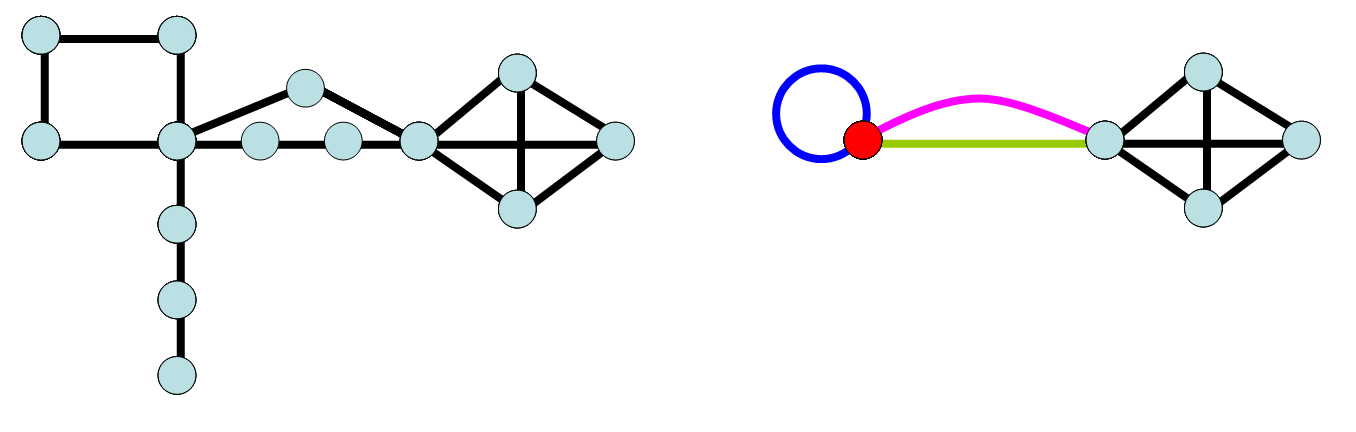
\includegraphics[height=50mm]{mln_reduction_v0.png}
\end{center}
\caption{A graph $G$ and the reduced graph $G''$. A black edge is of weight 1, a red one of weight 2, a green one of weight 3, and a purple one of weight 4. A red vertex denotes it is attached to a leaf by an edge of weight 3.}
\end{figure}

We now claim that $f$ is extendible to an isomorphism between $G_1$ and $G_2 \Leftrightarrow f$ is a coloured isomorphism between $G_1''$ and $G_2''$. 

If $f$ is extendible to an isomorphism between $G_1$ and $G_2$, then as our reduction process is isomorphism invariant, trivially $f$ will be a coloured isomorphism between $G_1''$ abd $G_2''$.

On the other hand, if $f$ is a coloured isomorphism between $G_1''$ and $G_2''$, then we can extend $f$ to an isomorphism over all of $G_1$ and $G_2$. To see this, note that the isomorphism type of a path of length $l$ is entirely characterized by its length. Hence if $f$ is a coloured bijection between $G_1''$ and $G_2''$, then by extending this bijection $f'$ along the paths, we create a full bijection between $G_1$ and $G_2$. Hence $f$ is extendible to an isomorphism over the whole graphs.







So by reducing $G_1$ and $G_2$ to $G_1''$ and $G_2''$, and testing if $f$ is an isomorphism between the reduced graphs, we indeed can decide whether or not $f$ is extendible to an isomorphism of the whole graphs.

Reducing the graphs takes $O(m)$ time, where $m$ is the number of edges in $G_1$. 

Testing if $f$ is a coloured isomorphism between $G_1''$ and $G_2''$ takes time $O(m''+n''^2)$, where m is the number of edges in $G_1''$ and $n$ is the number of vertices in $G_1''$. Since we decrease the number of edges in $G_1$ to create $G_1''$, we know $m''\leq m \leq n^2$. Likewise $n''^2 \leq n^2$, so this step takes time $O(n^2)$.

Putting this all together, the algorithm runs in time $O(n^2)$, and correctly decides whether or not $f$ is extentible to an isomorphism over the entire graphs.

\end{proof}

We can now prove our main result:

\begin{thm} Graph Isomorphism, parameterized by max leaf number, is fixed-parameter tractable.
\label{thm:mln_fpt}
\end{thm}
\begin{proof}

Given $G_1$ and $G_2$, each of max leaf number $k$:

Find $S=\{v\in V(G_1): \Delta(v)\geq 3\}$ and $T=\{v\in V(G_2):\Delta(v) \geq 3\}$. If $|S| \neq |T|$, then reject.

If $|S|=|T|=0$, then $\Delta(G)\leq 2$, so $G_1$ and $G_2$ are planar. In this case, use the planar isomorphism test of Datta et al. \cite{Datta09} to test for isomorphism in time $O(n)$.

Otherwise, loop through all possible bijections $f$ between $S$ and $T$, and use Claim \ref{mln_extend_iso_n2} to test if each is extendible to an isomorphism of the entire graph. If this is true for any of the bijections $f$, accept. Otherwise, reject.


Since $G_1\cong G_2 \Leftrightarrow$ at least one of these bijections $f:S\rightarrow T$ can be extended to a full isomorphism between the graphs, this algorithm will have the correct output.

Finding the set of vertices with degrees greater than or equal to 3 can be done in time $O(n^2)$ by counting the number of edges adjacent to each vertex. 

By Claim \ref{mln_subdiv} we know that $|S|\leq 4k-6$, so there are at most $(4k-6)!$ bijections to test. By Claim \ref{mln_extend_iso_n2} each bijection can be tested in time $O(n^2)$, so overall this algorithm takes time $O((4k-6)!n^2)$.

Hence graph isomorphism over graphs of max leaf number $k$ can be decided in time $O((4k-6)!n^2)$, so $(\GISO, $max leaf number$)\in \FPT$.






\end{proof}


This is our first fixed-parameter tractability result for $\GISO$.










\section{Vertex Cover Number}



We can extend the arguments used in the previous section to show $\GISO$ is also $\FPT$ when parameterized by vertex cover number. This result is subsumed by the fact that graph isomorphism is $\FPT$ when parameterized by the size of the smallest feedback vertex set \cite{Kratsch09}, so we only provide an outline of the proof.




Given a graph $G$, a vertex cover of $G$ is a set of the vertices $S \subseteq V(G)$ such that every edge in the graph is adjacent to $S$. The vertex cover number of a graph $G$, denoted $\vcn (G)$, is the minimum size of a vertex cover of $G$.

\begin{figure}[h]
\begin{center}
\leavevmode
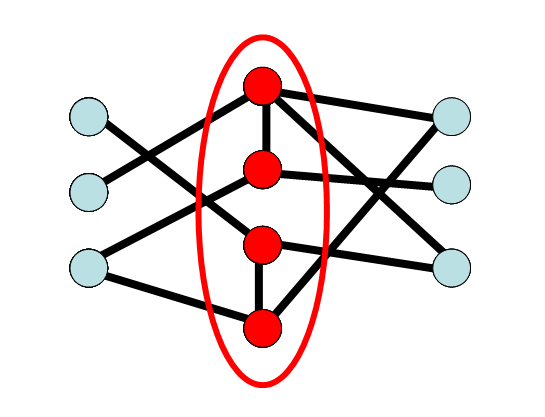
\includegraphics[height=60mm]{Vertex_Cover_Definition.png}
\end{center}
\caption{The red vertices form a vertex cover of this graph.}
\label{fig:image_2}
\end{figure}



Any vertex cover $S$ is also a feedback vertex set, since removing $S$ removes all edges from the graph, making the graph acyclic. Hence this result has been subsumed by Kratsch and Schweitzer's result that $(\GISO, $ minimum feedback vertex set size$)\in\FPT$ \cite{Kratsch09}.


 The following fact is key to creating an $\FPT$ algorithm for $\GISO$ parameterized by vertex cover number:


\begin{claim} If a graph $G$ has $\vcn(G)=k$, then there are at most $2^k$ different vertex covers of $G$ of size $k$. Furthermore, these vertex covers can be enumerated in time $O(2^{k} n)$.

\label{clm_vcn_enumerable_fpt}
\end{claim}

\begin{proof} See Flum and Grohe \cite{FlumGrohe} Chapter 1.

Pick an edge $e = (v,w) \in E(G)$. Then any vertex cover $S$ must contain $v$ or $w$. Define $A_S=\{ e \in E(G) : e$ is adjacent to $S  \}$. Consider $G'_{\{v\}}=G-A_{\{v\}}$, the graph obtained by deleting the edges of $A_{\{v\}}$ from $G$. Observe that $v$ is in a vertex cover of size $k$ if and only if $G'_{\{v\}}$ has vertex cover number $k-1$. This gives a recursive algorithm for enumerating all vertex covers of size $k$ of $G$ (for details see \cite{FlumGrohe}).


\end{proof}


Any isomorphism between graphs must preserve vertex covers. As in the last section, this allows us to create an algorithm which searches through all partial isomorphisms between all possible vertex covers of either graph, and tests whether or not each is extendible to a full isomorphism. For each of these partial isomorphisms, we can quickly check whether or not it is extendible to the rest of the graph:


\begin{claim} Suppose we are given graphs $G$ and $H$ with $\vcn(G)=\vcn(H)=k$, two minimal-sized vertex covers $S$ and $T$ of $G$ and $H$, respectively, and a partial isomorphism $f:S \rightarrow T$ over the vertex covers. 

Then, one can decide whether or not there exists an isomorphism $g:G \rightarrow H$ which extends $f$ in time $O(n)$.
\label{clm_vcn_extendable_n}
\end{claim}

\begin{proof} 

Since $S$ and $T$ are vertex covers, there cannot be any edges in the subgraphs induced by $V(G)-S$ and $V(H) -T$. Therefore every edge of the graph is either (1) from $S$ to $S$  or (2) from $S$ to $V(G)-S$.  Since we know that $f$ preserves the edge relation in case (1), to extend the isomorphism we simply need to preserve the edges in case (2).

Label the vertices of $S$ from $1$ to $k$ in an arbitrary order. For each vertex $v\in V(G)-S$, colour that vertex with the tuple $b_v = (b_1 , b_2, ... , b_k)$, where $b_i = 1$ if $v$ is adjacent to vertex $i$ in $S$ and $b_i = 0$ otherwise.  This colouring captures which vertices of $S$  the vertices of $V(G)-S$ are adjacent to. Colour the vertices of $w\in V(H)-T$ likewise with the tuples $b_w = (b_1 , b_2, ... , b_k)$, where $b_i = 1$ if $w$ is adjacent to $f(i)$ and $b_i = 0$ otherwise.


\begin{figure}[h]
\begin{center}
\leavevmode
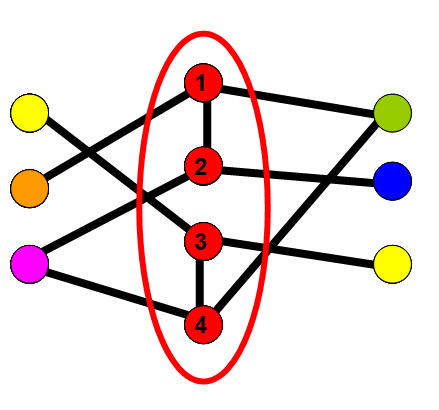
\includegraphics[height=60mm]{Vertex_Cover_colouring_v1.png}
\end{center}
\caption{A colouring of the vertices outside the vertex cover as decribed in Claim \ref{clm_vcn_extendable_n}.}
\label{fig:three}
\end{figure}



Consider the multisets $A=\{\{b_v : v \in V(G)-S  \}\}$ and $B=\{\{b_w : w \in V(H)-T  \}\}$. If $A=B$, then there is an isomorphism between the graphs which extends $f$. Indeed, it suffices to take the map $g: V(G) \rightarrow V(H)$ where $g(v)=f(v)$ for $v\in S$, and $g$ is any colour-preserving bijection between $V(G)-S$ and $V(H)-T$. Alternatively, if $A\neq B$ , then there is no isomorphism extending $f$ between $G$ and $H$ because there is no colour-preserving bijection between $V(G)-S$ and $V(H)-T$.


\end{proof}

From this point onwards, the proof that $(\GISO, $ vertex cover number$)\in\FPT$ follows analogously to Theorem \ref{thm:mln_fpt}.



















\chapter{Crossing Number}

One of the fundamental parameters for which $\GISO$ is not known to be $\FPT$ is genus. In this chapter we attempt to address a parameter related to genus, the crossing number. Although we do not show that $\GISO$ is $\FPT$ parameterized by crossing number, in our explorations we provide some evidence that the problem might be $\FPT$ reducible to isomorphism parameterized by the path-width of the graph.

\section{Introduction}



Given a graph $G$, a \emph{drawing} of $G$ into the plane $\Re ^2$ is a pair of maps $ (f: V(G) \rightarrow \Re ^{2}, \gamma : E(G) \rightarrow \{ \gamma _{e}:[0,1] \rightarrow \Re ^{2} \} ) $ such that:

1. $f(v)=f(w) \Rightarrow v=w$, that is, $f$ maps the vertices to distinct points in $\Re ^2$

2. If $e=(v,w)$, then $\gamma_e$ is continuous, $\gamma _{e}(0) = f(v)$ and $\gamma _{e}(1) = f(w)$, so the curve starts at $v$ and ends at $w$

3. At most two curves intersect at any given point in $\Re ^2$, except at the vertex points $\{f(v):v\in V(G)\}$.


The \emph{crossing number} of a graph $G$ is the minimum number of edge crossings (that is, points of intersection between the maps $\{ \gamma _{e}: e \in E(G) \}$  not at the vertex points) in any drawing of $G$. For instance, the crossing number of any planar graph is 0, and the crossing number of $K_{3,3}$ is 1. We denote the crossing number of $G$ by $\cross (G)$.

Clearly the crossing number of a graph is greater than or equal to the genus of the graph. Given a graph with crossing number $k$, consider a drawing of the graph with $k$ crossings, and create a surface $S$ which is the same as $\Re ^2$, but with $k$ small ``donut holes" located at the intersection points of the edges. The $G$ can be embedded in $S$ without any edge crossings, indicating that the genus of $G$ is less than or equal to $k$.
 
Graphs with small crossing number are ``nearly" planar in the sense that any graph of crossing number $k$ can be turned into a planar graph by deleting only $k$ edges. (This is trivial, because given a drawing of $G$ with $k$ crossings, we can simply remove one edge at each of the $k$ crossing points of the drawing to create a planar graph). Hence we say that graphs with crossing number $k$ have ``edge deletion distance"  $k$ away from planar graphs.

Graph isomorphism is known to be in $\P$ over planar graphs \cite{HopcroftWong74}. It is known that in some circumstances, having low edge deletion distance from a set of graphs with a poly-time isomorphism test does result in an efficient isomorphism algorithm:


\begin{claim} [From Kratsch and Schweitzer \cite{Kratsch09}] Suppose a graph class $C$ is characterized by a finite number of forbidden induced subgraphs
$H_1, . . . , H_l$. If the coloured graph isomorphism problem for graphs from $C$
is in $\P$, then the coloured graph isomorphism problem, parameterized by the vertex
deletion distance from $C$, is fixed-parameter tractable.
\label{clm:kratsch_del_dist}
\end{claim}


\begin{proof}See Theorem 1 from \cite{Kratsch09}. 

The basic idea is that, given two graphs $G_1$ and $G_2$, the algorithm finds a minimal deletion set $S$ of size $k$ in $G$ and a forbidden induced subgraph $H$ of $G_2$. Any isomorphism must map some vertex in $S$ to some vertex in $H$. The algorithm branches on all possible vertex pairs $(s,h):s\in S$ $h\in H$ and tries each of these as a possible partial isomorphism between the graphs. 

To see if the partial isomorphism from $s$ to $h$ can be extended to the remaining graph, the algorithm uses a similar technique to the one used in our proof of the fixed parameter tractability of vertex cover number. The algorithm removes $s$ from $G_1$ and recolours each $v\in V(G)$ of colour $c$ by the ordered pair $(c, b)$, where $b$ is 1 if $v$ is adjacent to $s$ and 0 otherwise. This colouring captures the adjacencies of s while removing s from the graph. The algorithm colours $G_2$ analogously. Then, the partial isomorphism is extendible to the rest of the graph if and only if the recoloured graphs are isomorphic (where the isomorphism respects colours). 

Note that removing $s$ and $h$ from their respective graphs reduces the vertex deletion distance from $C$ to $k-1$. Hence by removing these vertices and recursing, the recursion tree is bounded in the size of $k$, leading to an $\FPT$ algorithm.

\end{proof}



\begin{cor}
Suppose a graph class $C$ is characterized by a finite number of forbidden induced subgraphs
$H_1, . . . , H_l$. If the coloured graph isomorphism problem for graphs from $C$
is in $\P$, then the coloured graph isomorphism problem, parameterized by the {\bf edge}
deletion distance from $C$, is fixed-parameter tractable.
\end{cor}
\begin{proof}
Note that a graph of edge deletion distance $d$ from $C$ also has vertex deletion distance $\leq d$ from $C$. Indeed, suppose that we can remove $d$ edges from $G$ to create $G'\in C$. Starting with $G$, remove one vertex from each of those edges to create $G''$. Now $G''$ is a subgraph of $G'$, and since $C$ is characterized by forbidden induced subgraphs, $G''$ is in $C$ as well.
\end{proof}

We know that graphs of crossing number $k$ are edge deletion distance $k$ away from planar graphs, and that coloured graph isomorphism is in $\P$ over planar graphs \cite{HopcroftTarjan72} \cite{HopcroftWong74}\cite{Grohe10}. If planar graphs were characterized by a finite number of forbidden subgraphs, this would trivially prove the fixed-parameter tractability of $\GISO$ with respect to crossing number. Elementary graph theory, however, tells us this is not the case. By Kuratowski's Theorem, we know that a graph is planar if and only if it excludes any subdivision of $K_5$ or $K_{3,3}$ as a subgraph, or equivalently if it excludes $K_5$ and $K_{3,3}$ as a minor \cite{Harris08}. So the class of planar graphs is characterized by an infinite number of forbidden subgraphs, and a finite number of forbidden minors. If we could somehow modify Kratsch and Schweitzer's theorem to accomodate for graph minors, then this would immediately imply our desired result.

Another simple way of modifying Kratsch and Schweitzer's algorithm is as follows. Suppose that graphs $G_1$ and $G_2$ have crossing number $k$. What if the number of edges whose removal decreases the crossing number were bounded as a function $f$ of $k$? If $E_1$ is a set of edges of $G_1$ of size $k$ whose deletion yields a planar graph, and $E_2$ is the set of edges whose removal decreases the crossing number of $G_2$, then any isomorphism between the graphs must map some edge of $E_1$ to some edge of $E_2$. We could then try all possible mappings between edges $(e_1,e_2), e_1 \in E_1$ $e_2 \in E_2$ and recurse on the remaining graph, precisely analogously to Claim \ref{clm:kratsch_del_dist}. Since there would only be $kf(k)$ pairs to try at any stage in the recursion, and the recursion tree has depth $k$, this would create a bounded recursion tree and thus show $(\GISO,$ crossing number$)\in\FPT$.

However, in general, the number of edges whose removal decreases the crossing number is not bounded by a function of $k$. In fact, there exist infinite families of graphs known as $k$-crossing-critical graphs for which removing any edge decreases the crossing number.

A graph $G$ is called \emph{k-crossing-critical}, denoted KCC, if 

1. $\cross(G)\geq k$

2. $\forall e \in E(G)$, $\cross(G-e)<k$, where $G-e$ denotes the graph obtained by removing $e$ from $G$. 

KCC graphs are the subject of contemporary combinatorial research. There exist several known infinite families of KCC graphs such that, for each $n_0$, there exists a KCC graph in the family of size $n\geq n_0$ \cite{Hlineny08}. For instance, the ``crossed fence" family of KCC graphs consists of the following construction: Create a square lattices of points in a diamond shape of width $k$ and wrap it around a cylinder (this is the ``fence"). To one side of the fence pick two vertices distance $> k$ apart and attach a node $w_1$ to each of them. Do likewise to create a node $w_2$ on the botton side of the fence, and then ``cross" the fence by connecting $w_1$ and $w_2$.  Hlin\u{e}n\'{y} showed that this construction is indeed $k$-crossing critical \cite{Hlineny08}. 


\begin{figure}[b!]
\begin{center}
\leavevmode
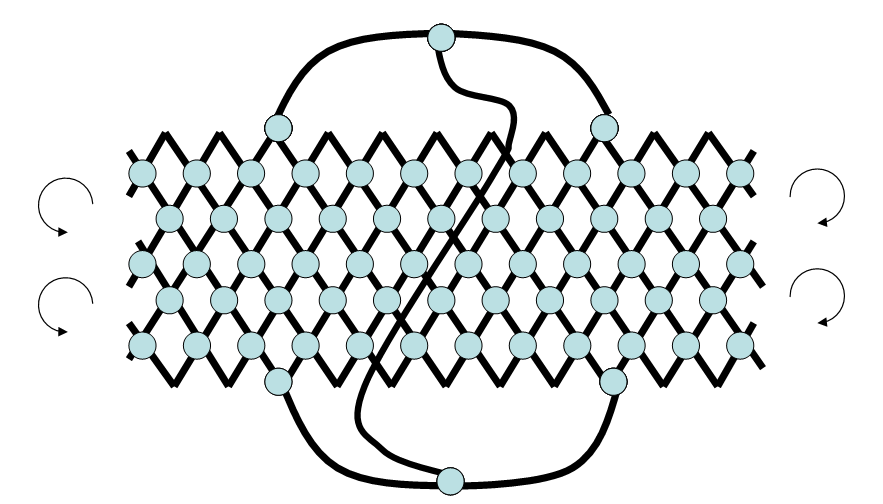
\includegraphics[height=69mm]{Crossed_Fence_v2.png}
\end{center}
\caption{A Crossed Fence 6-crossing critical graph \cite{Hlineny02}. The left and right edges of the graph are attached as if wound around a cylinder.}
\label{fig:four}
\end{figure}

 Note that other infinite families of KCC graphs can be created using the ``M\"{o}bius strip" method, which uses a fence or grid and, instead of crossing the fence, adds a half-twist to the fence \cite{Hlineny08}. 


Work is currently being done to better understand the structure of KCC graphs. There are several open conjectures in the field, including:

\begin{conj} If $G$ is $k$-crossing critical, then the number of vertices of odd degree greater than 6 is bounded as a function of $k$ \cite{Hlineny08}.
\end{conj}


\begin{conj}  If $G$ is $k$-crossing critical, then the maximum degree of the graph $\Delta(G)$ is bounded as a function of $k$  \cite{RichterSalazar08}.
\label{conj:bounded_cn_bounded_deg}
\end{conj}

\begin{conj}
If $G$ is $k$-crossing critical, then the bandwidth of the graph is bounded as a function of $k$ \cite{RichterSalazar08}. If proven, this would imply Conjecture \ref{conj:bounded_cn_bounded_deg} as well, since graphs of bandwidth $k$ have degree at most $k$.
\end{conj}



Many facts about KCC graphs have been proven, the most relevant of which is the following fact: 

\begin{thm} [From Hlin\u{e}n\'{y} 2002 \cite{Hlineny02}] Suppose a graph $G$ is $k$-crossing critical. Then the pathwidth of $G$ is bounded by a function of $k$. Specifically, the path-width of $G$ is most $2^{f(k)+1}-2$, where $f(k) \leq 6 · (72 \log_{2} k + 248) · k^3$.
\label{kcc_implies_pw}
\end{thm}

Note that $G$ must be $k$-crossing-\emph{critical} in order to have bounded pathwidth. Graphs which only have crossing number $k$ need not have bounded pathwidth. Indeed, there are planar graphs, such as binary trees, which have arbitrarily high pathwidths but have crossing number 0. 

Suppose $\GISO$ were $\FPT$ when parameterized by path-width. Then, by Theorem \ref{kcc_implies_pw},
 $(\GISO,$ crossing number$)$ would be $\FPT$ when restricted to $k$-crossing critical graphs. A natural question is whether or not we could extend this isomorphism algorithm for KCC graphs to work for all graphs of crossing number $k$. If so, then we would show that $(\GISO,$ path-width$)\in\FPT\Rightarrow (\GISO, $ crossing number$)\in\FPT$.

In the next section we present evidence that this might be the case. We create an algorithm which canonically decomposes graphs of crossing number $k$ into planar and $k$-crossing-critical components. This algorithm is isomorphism-invariant, so could form the basis of an $\FPT$ reduction between crossing number and pathwidth. We explore this idea, and the difficulties that arise in turning this into a proven reduction.



\section{Reducing Crossing Number to Pathwidth}

We would like to create a $\FPT$ reduction from crossing number to pathwidth. To do so, we suppose that $\GISO$ is in $\FPT$ when parameterized by pathwidth. Our goal is to create an isomorphism algorithm for crossing number using the isomorphism algorithm for pathwidth as a black box. If we are able to do so, then we will show that $(\GISO,$ pathwidth$)\in \FPT \Rightarrow (\GISO,$ crossing number$)\in \FPT$. This is essentially a parameterized Cook reduction between the problems, which transforms an instance of the problem into at most $f(k)n^c$ instances of the pathwidth problem, rather than a parameterized Karp reduction (which we defined previously).


From Theorem \ref{kcc_implies_pw}, we know that all $k$-crossing critical graphs have bounded path-width as a function of $k$, so we can solve $\GISO$ efficiently for these $k$-crossing critical graphs. If we could decompose our graphs of crossing number $k$ into their ``critical" and ``planar" components, then we could easily solve graph isomorphism separately on each of these components, and perhaps combine the results to test for isomorphism on the entire graphs.

We now provide a fixed-parameter tractable  algorithm which creates a canonical (that is, isomorphism-invariant) decomposition of a graph into planar and KCC components. A key fact that we use in the proof is that testing whether the crossing number of a graph is less than or equal to $k$ is fixed parameter tractable with respect to $k$ \cite{Grohe01}; in fact, it can be done in linear $\FPT$ time \cite{Kawarabayashi07}.


% canonical graph decomposition algorithm
\begin{algorithm}[h]
\SetAlgoNoLine
\KwIn{A graph $G$ of crossing number $k$}
\KwOut{ A partition of the edges of $G$ into sets $E_1$, $E_2$, ... $E_l$ such that $l\leq k$

  }

\Repeat{$|E(G)|==0$}{

	$E_i = \{e\in E(G) : \cross(G-e) = \cross(G)\}$ ;

	\If{$|E_i| == 0$ OR $|E_i| == |E(G)|$}{$E_i = E(G)$;}
	
	

	$E(G) = E(G)-E_i$;
	

}
\caption{Canonical Decomposition Algorithm for graphs of Crossing Number $k$}
\label{alg:cn_decomp}
\end{algorithm}

\begin{thm}{Algorithm \ref{alg:cn_decomp} produces a partition of the edges of $G$ such that all the graphs $(V(G), E_i)$ are planar except potentially $(V(G), E_l)$, which could be $k'$-crossing-critical for $k'\leq k$}.

\end{thm}
\begin{proof}

Given $G$ of crossing number $k$:

Let's describe what happens to $G$ in step $i$ of the algorithm, when $\cross(G)=k_i$.

Consider $E_i= \{e\in E(G) : \cross(G-e) =k_i\}$.

Note that for any edge $e$, $\cross(G-e)\leq k_i$, since removing any edge cannot increase the crossing number.

Hence if $|E_i| ==0$, then for each edge $\cross(G-e)<\cross(G)$, so $G$ must be $k_i$-crossing critical. In this case, by setting $E_i = E(G)$, we ensure the algorithm terminates before starting the next iteration, and the algorithm terminates with a $k_i$-crossing-critical graph.

Now, if $|E_i|==|E(G)|$, then removing any edge from $G$ does not affect its crossing number. This immediately implies that $G$ is planar. (To see this, suppose by way of contradiction that $\cross(G) >0$. Consider any drawing of $G$ with a minimal number of crossings. At least one edge $e$ is crossed in this drawing. Then immediately we have $\cross(G-e) < \cross(G)$, yielding a contradiction.)  Again by setting $E_i = E(G)$ we ensure the algorithm terminates before beginning the next step.

We are now left with the third case, where $0<|E_i|<|E(G)|$. In this case, we will show that $(V(G), E_i)$ is planar. 

Consider $D$, the set of all drawings of $G$ with exactly $k_i$ crossings. Since $G$ has crossing number $k_i$, $D$ is nonempty. Furthermore, for each edge $e \in E_i$, $e$ cannot be crossed in any drawing in $D$ (otherwise, removing $e$ from the graph would create a drawing with $<k_i$ crossings, which is a contradiction). Hence in any drawing in $D$, every edge in $E_i$ is not crossed. This implies any drawing in $D$ is a planar drawing of the graph $(V(G), E_i)$, so since $D$ is nonempty,  $(V(G), E_i)$ is planar.

We have now established that every graph in the sequence is either planar or crossing-critical, and that if the graph is crossing-critical, then it is the last graph in the sequence. Furthermore, this algorithm is trivially isomorphism invariant, as no arbitary choices are made in the algorithm, and the crossing number of a graph is isomorphism invariant. Hence this algorithm does produce a canonical decomposition of the graph efficiently. 

We now need to show that the algorithm terminates after at most $k$ rounds. If we ever reach $|E_i|==|E(G)|$ or $|E_i|==0$, then we terminate on the next round, so we are done. So we only need to look at what happens when  $0<|E_i|<|E(G)|$.  In this case,  we remove a subset of the edges from $G$ to create a new graph $G'$, with $\cross(G')\leq cross(G)$. So at the end of this step, either $\cross(G')=\cross(G)$ or $\cross(G')<\cross(G)$. We show that only the latter case is possible.

If $\cross(G')=\cross(G)$, then we know that $G'$ must be $k_i$-crossing critical, hence the algorithm must terminate in the next iteration. To see this, suppose by way of contradiction that $G'$ is not $k_i$ crossing critical. Then there is some edge $e$ in $G'$ such that $\cross(G'-e)=\cross(G')=\cross(G)$. Since we know that $e$ was not removed in this step, removing $e$ from $G$ must decrease its crossing number. Hence there is a drawing $d$ of the graph $G-e$ with less than $k_i$ crossings. But note that $d$ is also a drawing of the graph $G'-e$ with less than $k_i$ crossings. Hence $\cross(G'-e)<k_i$, yielding a contradiction. 


Therefore we know that $\cross(G')<\cross(G)$, so the crossing number strictly decreases at each round. Hence the algorithm terminates after at most $k$ iterations.

Since finding $E_i$ and removing it from the graph can be done in time $O(f(k)mn)$, this means that the algorithm runs in time $O(kf(k)mn)$. Hence this is indeed an $\FPT$ algorithm.

\end{proof}

We therefore have an $\FPT$ algorithm to canonically decompose a graph of crossing number $k$ into at most $k$ planar graphs and at most one crossing critical graph. Since we are assuming $\GISO$ is $\FPT$ with respect to pathwidth in this section, we know that we can solve isomorphism in $\FPT$ time on each of these components individually. Clearly if $G _1 \cong G_2$, then both graphs must have isomorphic decompositions, so testing these individual isomorphisms is a necessary condition for isomorphism between these graphs. However, this condition is not sufficient to ensure isomorphism between the graphs, as the example in Figure \ref{fig:crosnum_fail} demonstrates. Hence we need a stronger condition to ensure isomorphism between the graphs. 


\begin{figure}[b]
\begin{center}
\leavevmode
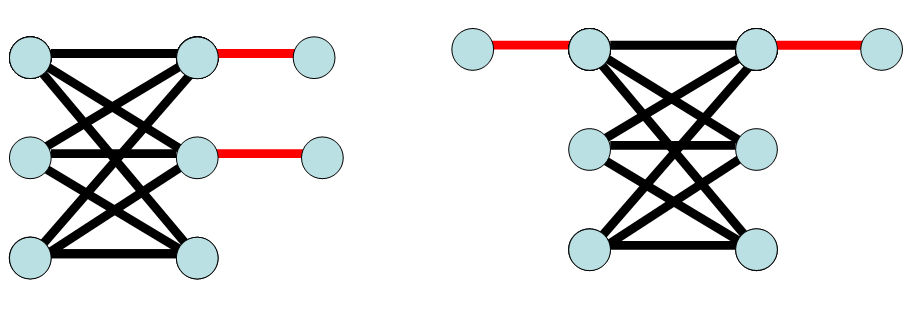
\includegraphics[height=50mm]{NonIso_Same_Decomp_v0.png}
\end{center}
\caption{Two non-isomorphic graphs of crossing number 1 which have the same canonical decomposition into $K_{3,3}$ (black edges) and two $K_2$ graphs (red edges)}
\label{fig:crosnum_fail}
\end{figure}



Given a graph $G$, the automorphism group of $G$, denoted $Aut(G)$, is the set of automorphisms of $G$. (Recall that an automorphism of a graph is an isomorphism from the graph to itself). The orbit of a vertex $v\in V(G)$, denoted $O_v$  is the set $\{w \in V(G)| \exists f\in Aut(G) : f(v)=w\}$. The set of orbits of the automorphism group form an equivalence relation on the vertices of $G$, because if $w\in O_v$, then $v\in O_w$ because isomorphisms are invertible. The orbits of the automorphism group of a graph convey information about the structure of $Aut(G)$, but they do not provide enough information to fully describe $Aut(G)$. For instance, the orbits of $K_n$ and $C_n$ are both the entire graph, but the automorphism group of the former is much larger than that of the latter.

Note that if we can test for coloured graph isomorphism between two graphs efficiently, then we can also efficiently label the vertices of the graph by their orbits. Suppose we are given two coloured graphs $G_1$ and $G_2$, and we can test that $G_1$ and $G_2$ are isomorphic in time $O(f(k)n^c)$. If we find that $G_1 \cong G_2$, then we can label the graphs as follows: 

For each vertex $v\in V(G_1)$, test, for each $w\in V(G_1)$, whether or not $G_1 - v \cong_{\CGISO} G_1 - w$, where $G_1 - x$ has been recoloured by giving vertex $y$ colour $(c,1)$ if $y$ is adjacent to $x$ and colour $(c,2)$ otherwise, where $c$ is the original colour of $y$. Clearly $G_1 - v \cong_{\CGISO} G_1 - w \Leftrightarrow w\in O_v$. So this allows us to label the orbits of $G_1$ with labels 1...$k$, where $k$ is the number of distinct orbits of the graph. We then colour $G_2$ with the same colours 1...$k$ by giving vertex $w\in V(G_2)$ the same colour as any $v\in V(G_1)$ such that $G_1 - v \cong_{\CGISO} G_2 - w$. Since $G_1 \cong G_2$, these are the same graph, so the orbits will be labelled correspondingly. Overall, this can be completed in time $O(f(k)n^{c+2})$, which is also an efficient algorithm. We can therefore label the orbits of two isomorphic graphs efficiently. 




Given a graph of crossing number $k$, we've seen that we can canonically decompose it into at most $k$ graphs, each of which admits an $\FPT$ isomorphism test. Also, we can easily label the orbits of the automorphism groups of each of these subgraphs efficiently. If we're given two graphs $G_1$ and $G_2$  which have isomorphic canonical decompositions, then one way to distinguish non-isomorphic graphs from one another is to test whether the orbits of each of these graphs interact in the same way. We can do this by colouring each of the graphs by the orbits of their automorphism groups, and then taking the  intersection of these colourings. This leads us to a colour refinement algorithm, Algorithm \ref{alg:orbitrefinement}, which attempts to create a colouring of the orbits of $G_1$ and $G_2$ based on the orbits of its constituent components.




\begin{algorithm}[h]
\SetAlgoNoLine
\KwIn{Graphs $G_1$ and $G_2$ of crossing number $k$.}
\KwOut{A colouring of $G_1$ and $G_2$ .}
$index$ = $|G|$; 

Canonically decompose $G_1$ and $G_2$ into graphs $E_1$...$E_l$ and $F_1$...$F_l$ respectively using Algorithm \ref{alg:cn_decomp}.

Check for each $i=1$...$l$ that $E_i \cong F_i$, otherwise return;

\Repeat{index==0;}{   

For each $i=1$...$l$ label the orbits of $E_i$ and $F_i$ correspondingly as above.

Colour each vertex $v\in V(G_1)$ by $(c, c_1, c_2, $...$c_l)$ where $c$ is the old colour of vertex $v$ and $c_i$ is the orbit label of vertex $v$ in graph $E_i$. Do likewise for $G_2$.

$index-$$-$; }
\caption{An orbit refinement algorithm for graphs with isomorphic canonical decompositions}
\label{alg:orbitrefinement}
\end{algorithm}

Note that the colouring produced by this algorithm is strictly refined at each stage, so it will take at most $n$ iterations to stabilize. So this algorithm is indeed a tractable algorithm for the problem, since we are assuming $(\CGISO,$ path-width$)\in \FPT$. Also note that this algorithm successfully distinguishes the graphs in Figure 4.2.

This algorithm clearly produces a colouring which is compatible with a colouring of the orbits of the automorphism groups of $G_1$ and $G_2$, because since $G_1$ can be decomposed edgewise into $E_i$, $i=1$... $l$, then $Aut(G_1) \subseteq \displaystyle\bigcap_{i\in [1,...,l]} Aut(E_i)$, which implies $O_v \subseteq \displaystyle\bigcap_{i\in [1,...,l]} O_v(E_i)$, where $O_v(E_i)$ is the orbit of $v$ in subgraph $E_i$. So clearly this algorithm does not refine the colouring beyond the orbits of $Aut(G_1)$.

If the colouring produced by this algorithm is actually a colouring of the orbits of $Aut(G_1)$ and $Aut(G_2)$, then testing for isomorphism between the graphs becomes fixed-parameter tractable under our assumptions. Give $G_1$ and $G_2$ of crossing number $k$, we could colour them using Algorithm \ref{alg:orbitrefinement}. If the multisets of colours contained in each graph are not equal, then clearly the graphs are not isomorphic. Otherwise, pick $v\in V(G_1)$ and $w\in V(G_2)$ of the same colour such that $\cross(G_1-v)<k$. Then clearly $G_1 \cong G_2 \Leftrightarrow G_1-v \cong G_2-w$ , where the colouring of the graphs $G_i - x$ are refined to convey whether or not the vertices are or are not adjacent to $x$, as above.  If the new graphs are isomorphic, then repeat. This can only continue at most $k$ steps since the crossing number decreases at each stage. Hence this would produce an algorithm to test for isomorphism between the graphs in time $O(f(k)n^c)$. 


Ergo if Algorithm \ref{alg:orbitrefinement} actually colours the orbits of $G_1$ and $G_2$, then we know that $(\CGISO,$  path-width$)\in \FPT \Rightarrow (\GISO,$ crossing number$)\in \FPT$.




\section{Future work to be done}


Unfortunately, it's not clear that this algorithm will properly colour the orbits of $Aut(G_1)$ and $Aut(G_2)$. This algorithm does not work for general edge decompositions of graphs. For instance, consider the edge decomposition of the graph in Figure \ref{fig:edge_decomp_fails} into two copies of $C_7$, the 7-cycle:


\begin{figure}[h]
\begin{center}
\leavevmode
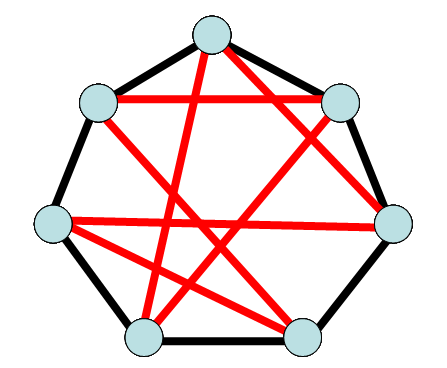
\includegraphics[height=50mm]{Crossing_Decomp_Alg_Fails_v0.png}
\end{center}
\caption{An edge decomposition into two copies (one red, one black) of $C_7$ showing that orbit Refinement does not work for generic edge decompositions.}
\label{fig:edge_decomp_fails}
\end{figure}

Clearly the orbits of the automorphism group of each subgraph is the entire graph, so Algorithm \ref{alg:orbitrefinement} would give this graph a single colour. However, the actual colouring of the orbits of the automorphism group of this graph uses 7 colours. So on general graph decompositions of $G$, Algorithm \ref{alg:orbitrefinement} does not produce a colouring of the orbits of $Aut(G)$. However, this example does not immediately show our algorithm is incorrect, since this particular edge decomposition is not an example of a canonical edge decomposition.

Hence if we want to prove that this algorithm is correct, we would need to leverage the fact that we are using our particular canonical decomposition algorithm. Any such proof would have to leverage a number of detailed topological facts, in a similar fashion to the planar isomorphism testings algorithms of Hopcroft, Tarjan and Wong \cite{HopcroftTarjan72} \cite{HopcroftWong74}. Here we leave open the question of whether or not this colour refinement algorithm works. 

Note that even if this colour refinement algorithm does not work, there could be other ways to leverage our canonical decomposition algorithm to prove $(\CGISO,$ path-width$)\in \FPT \Rightarrow (\GISO,$ crossing number$)\in \FPT$. A more sophisticated approach would be to directly mimic the planar isomorphism testing algorithm of Hopcroft, Tarjan and Wong \cite{HopcroftTarjan72} \cite{HopcroftWong74}. The planar isomorphism algorithm decomposes the graph into 2 and 3 connected components in a tree-like structure, then propagates the automorphism group constraints up the tree structure to determine isomorphism over the entire graph. In our case, our decomposition algorithm has a path-like structure to it, which could allow us to perform a similar propagation of automorphism group constraints to the entire graph. However, such an algorithm could not work exactly analogously to the Hopcroft Tarjan and Wong algorithm because our decomposition of the graph is over the \emph{edges} of the graphs rather than the vertices. This algorithm would be heavily topological in nature. Such an approach could be fruitful for future research.


















\chapter{Tree-Depth}

In this chapter we show that, if a certain conjecture holds, then graph isomorphism is fixed-parameter tractable with respect to tree-depth. We also provide several ideas as to how this conjecture could be proven. 

\section{Introduction }

A directed tree $T$ is a graph consisting of a root $r$ and a connected strongly acyclic graph (where strong acyclic means the graph is acyclic even if the directed edges are replaced by undirected edges) which is directed away from $r$. Given a tree $T$, the depth of $T$ is the length of the longest path from $r$ to any  vertex in the graph. A vertex $v$ is said to be an ancestor of vertex $w$ if there is a directed path from $v$ to $w$ in $F$. The closure of $T$, denoted $clos(T)$, is the undirected graph obtained by taking the symmetric transitive closure of $T$. In other words, it is the graph obtained by adding an undirected edge between two verticies $v$ and $w$ if and only if one is the ancestor of another in $T$.

 A directed forest is a graph whose connected components are directed trees. The closure of a directed forest is defined to be the closure of its connected components.

\begin{figure}[h]
\begin{center}
\leavevmode
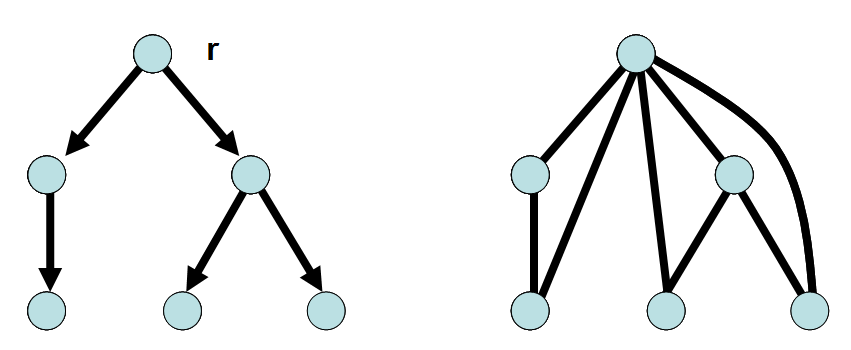
\includegraphics[height=50mm]{Closure_Forest_v2.png}
\end{center}
\caption{A tree $T$ and its closure.}
\end{figure}


A forest $F$ is said be a \emph{forest decomposition} of a graph $G$ if $G$ is a subgraph of $clos(F)$. The \emph{tree-depth} of $G$, denoted $td(G)$, is the minimum height of a forest $F$ which is a forest decomposition of $G$. 

\begin{figure}[h]
\begin{center}
\leavevmode
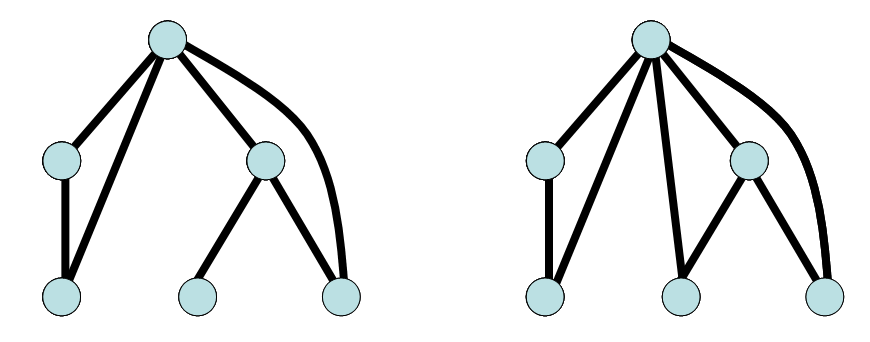
\includegraphics[height=50mm]{Tree_Decomp_v1.png}
\end{center}
\caption{A graph G and the closure of its tree decomposition.}
\label{fig:decomp}
\end{figure}


Tree-depth is also known as the \emph{minimum elimination tree height} or the \emph{vertex ranking number}. The parameter has been studied extensively in the area of factorization of sparse matrices (\cite{Heath91} via \cite{Manne91}). In this area, the nodes of the graph represent chunks of computational work, and the edges represent the dependencies between these computations. In this context, graphs of low tree depth are computations which are easily solvable by a parallel computation using an unbounded number of processors.

Tree-depth is a generalization of the vertex cover number of a graph. For any graph, $td(G)\leq \vcn(G)$. To see this, note that any graph of vertex cover number $k$ has a depth $k$ decomposition taken as follows: Order the vertices of a minimal vertex cover arbitrarily and place them in a path. At the bottom of the path, attach all remaining nodes of the graph. This is a tree of height $k$, and the closure of this tree contains all edges adjacent to the vertex cover, which by the defintion of the vertex cover must be a superset of the edges of the graph. Hence for any graph $G$, $td(G)\leq \vcn(G)$.

\begin{figure}[b]
\begin{center}
\leavevmode
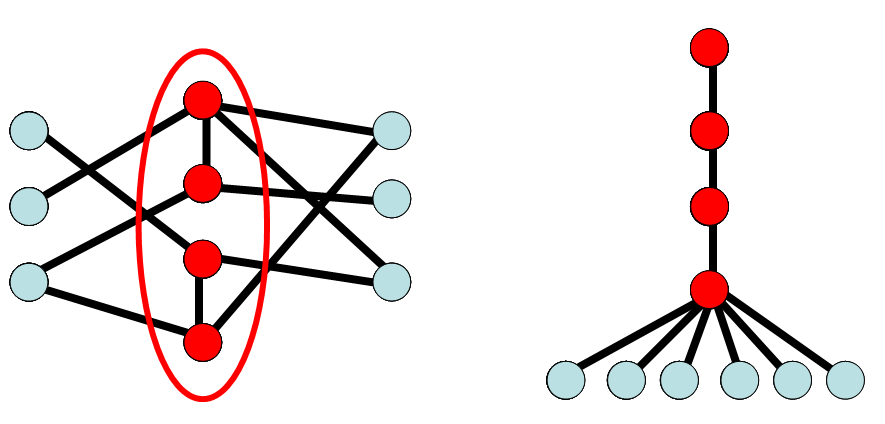
\includegraphics[height=50mm]{VCN_implies_TD_v0.png}
\end{center}
\caption{A graph of Vertex Cover Number $k$, and its forest decomposition of height $k$.}
\label{fig:vcn_implies_td}
\end{figure}

Likewise, path-width is a generalization of tree-depth, because for any graph $G$, $pw(G)\leq td(G)$, where $pw(G)$ is the path-width of $G$. To see this, given any graph $G$ of tree-depth $k$ consider a minimum height tree decomposition of $G$. Now take the bags of the path decomposition $X_i$ to be the sets of vertices on paths from the root of the tree decomposition to a leaf, taken in the order the leaves would be visited in a depth-first search. Then this is a valid path decomposition of $G$, with width $k$. Hence for any graph $G$, $pw(G)\leq td(G)$. So if $\GISO$ were $\FPT$ when parameterized by path-width, then it would trivially also be $\FPT$ parameterized by tree-depth. However $\GISO$ is not known to be $\FPT$ parameterized by path-width.




An alternative and equivalent definition of tree-depth provided by Ne\u{s}et\u{r}il and Ossona de Mendez \cite{Nesetril06} will prove very useful in constructing our algorithm:

\begin{claim} Let $G$ be a graph with connected components $G_1$, ..., $G_p$. 

Then $td(G)=\left\{  \begin{array}{ll}
  1 & \quad \mbox{if $|V(G)|=1$}\\
  1+\displaystyle\min_{v\in V(G)} td(G-v) & \quad \mbox{if $p=1$ and $|V(G)|>1$}\\
  \displaystyle\max_{i=1...p}td(G_i) & \quad \mbox{otherwise}\\ \end{array} \right\}$



\label{clm_td_iterative_defn}
\end{claim}
\begin{proof}
See Ne\u{s}et\u{r}il and Ossona de Mendez, Lemma 2.1 \cite{Nesetril06}.
\end{proof}


Tree-depth is also well-behaved with respect to the operation of taking minors.

\begin{claim}  If $H$ is a minor of $G$, then $td(H)\leq td(G)$ \cite{Nesetril06}.
\label{clm_td_minors}
\end{claim}
\begin{proof} [From Ne\u{s}et\u{r}il and Ossona de Mendez \cite{Nesetril06}]
Given a graph $G$ with a minimum height decomposition $F$: Suppose we contract an edge $(v,w)\in E(G)$ to create a graph $G'$. Then $(v,w) \in E(clos(F))$, so $v$ is an ancestor of $w$ in $F$. Consider the forest $F'$ obtained by identifying $v$ with its parent $p(v)$ . Then $G'\subseteq clos(F')$. Hence $td(G')\leq td(G)$.

\end{proof}

This fact can be used to show that we can test if a graph has tree-depth $d$ efficiently:


\begin{claim} Given a graph $G$, we can find the tree-depth of $G$ in time $O(f(d)n)$ for some function $f$, where $d=td(G)$. \cite{Bodlaender98}.
\label{clm_test_td_fpt}
\end{claim}
\begin{proof} Provided by Bodlaender et al. \cite{Bodlaender98}

Let $C_d=\{G: td(G)\leq d\}$. Then by Claim \ref{clm_td_minors} the class $C_d$ is closed under the operation of taking minors. Trivially the class $C_d$ does not contain all planar graphs, as it doesn not contain $P_{2^{d+2}}$, the path of length $2^{d+2}$. By a theorem of Bodlaender (which is a consequence of a theorem of Robertson and Seymour) any minor-closed class of graphs which does not contain all planar graphs has a linear time recognition algorithm \cite{Bodlaender93}. Hence given $G$ we can decide for each $d$ if $G\in C_d$ in time $O(g(d)n)$. By repeating this for $d=1$...$td(G)$, we can find the tree-depth of $G$ in time $O(f(d)n)$, where $f(d)=\displaystyle\sum\limits_{i=1}^{d} g(d)$.


\end{proof}

Note that underlying this result is a powerful theorem by Robertston and Seymour, which states that any proper minor closed class is characterized by a finite number of forbidden minors \cite{RobertsonSeymour}. This theorem is non-constructive, so the function $f(d)$ described above is not necessarily computable. In order to consider this algorithm to be $\FPT$, we need to relax our notion of fixed-parameter tractability to allow the function $f(k)$ to be non-computable. This relaxation of $\FPT$ is known as uniform $\FPT$ \cite{Downey95}, whereas requiring $f$ is be computable is known as strongly uniform $\FPT$. In this chapter we will only consider the uniform version of $\FPT$.







\section{A potential proof that $(\GISO ,$tree-depth$)\in\FPT$}


With the basic facts about tree-depth established, we can now work to create an algorithm which shows that graph isomorphism parameterized by tree-depth is in $\FPT$. The basic idea is to extend the logspace algorithm for tree isomorphism developed by Lindell \cite{Lindell92} to test for isomorphism over forest decompositions of a graph. 

For the moment assume that our graphs are connected; later we will show that our algorithm also works for disconnected graphs.

Lindell's algorithm works by establishing an ordering $<$ on the set of trees \cite{Lindell92}. In his algorithm, two trees $S$ and $T$ obey $S<T$ if

1. $|S|<|T|$, where $|S|$ denotes the number of nodes in $S$.

2. $|S|=|T|$ and $\#s < \#t$, where $\#s$ is the number of children of the root of $S$

3. $|S|=|T|$,  $\#s = \#t = k$ and $(S_1, S_2, ... ,S_k) < (T_1, T_2, ..., T_k)$ lexicographically, where we inductively assume that $S_1 \leq S_2 \leq ... \leq S_k$ and $T_1 \leq T_2 \leq ... \leq T_k$ are the ordered subtrees of $S$ and $T$ obtained by removing the roots of $S$ and $T$

Clearly if neither $S<T$ or $T<S$ then $S \cong T$. Alternatively, if $S<T$ or $T<S$ then $S$ and $T$ are not isomorphic \cite{Lindell92}. 

Our idea is to extend this ordering on trees to an ordering of the tree decompositions of a graph $G$. Recall that a tree decomposition of a graph $G$ consists of a tree $T$ over $V(G)$ and a subset $E(G)\subseteq E(clos(T))$. We say that two decompositions $T_1$ and $T_2$ are equivalent, denoted $T_1 \simeq T_2$, if their respective trees are isomorphic, and furthermore there is an isomorphism between the trees which preserves $E(G)$ as well. So in particular, an isomorphism between tree decompositions is also an isomorphism between the graphs.


To test for isomorphism, our algorithm finds a minimal decomposition of each graph. If the two graphs are isomorphic, then they have the same minimal decomposition. If two graphs are nonisomorphic, then they do not have the same minimal decomposition. We show that we can find this minimal decomposition efficiently, so this gives us an efficient test for graph isomorphism. We create this algorithm by defining an order on decompositions recursively in such a way that our recursion tree has depth and breadth bounded as a function of the tree-depth. 


\begin{figure}[t]
\begin{center}
\leavevmode
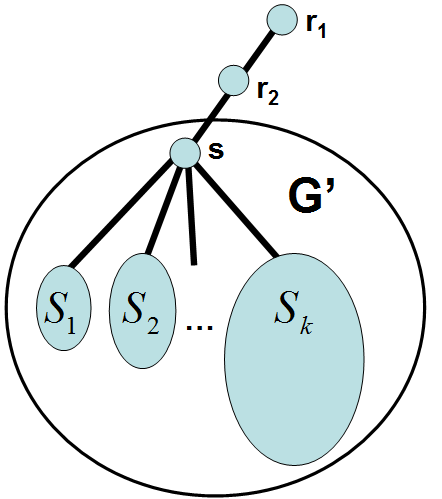
\includegraphics[height=70mm]{td_partial_decomp_v1.png}
\end{center}
\caption{A sub-decomposition of $G'$ with root $s$ and connected components $S_1...S_k$ of $G'-s$.}
\label{fig:td_sub_decomp}
\end{figure}



Suppose that we are given a connected graph $G$ with $td(G)=d$. We inductively define an ordering of (sub) tree decompositions of $G$ as follows:


Consider a connected subgraph $G'$ of $G$ of tree-depth $d'\leq d$. If $d'<d $ suppose that the root of the decomposition of $G$ is fixed, as well as the path of vertices to the root $r=r_1, r_2, ... r_{d-d'}$ in the entire decomposition of $G$ of length $d-d'$. Also assume that $G'$ is a connected component of $G-r_1-r_2-...-r_{d-d'}$.

Let $S$ and $T$ be two depth $d'$ decompositions of $G'$, with roots $s$ and $t$, respectively.


\newpage


We say that the decomposition $S$ of $G'$ is less than the decomposition $T$, denoted $S<T$, if one of the following conditions is satisfied:

1. $(E(r_1,s), E(r_2,s),...,E(r_{d-d'},s))<(E(r_1,t), E(r_2,t),...,E(r_{d-d'},t))$ lexicographically, where $E(x,y)=1$ if there is an edge from $x$ to $y$ and 0 otherwise. If $d=d'$, then we ignore this condition.

2. $E(r_i, s)=E(r_i,t)$ $\forall i=1...(d-d')$ and $\#s < \#t$, where $\#x$ is the number of connected components in $G'-x$.

3. $E(r_i, s)=E(r_i,t)$ $\forall i=1...(d-d')$, $\#s = \#t= k$, and \[(\chi(S_1), \chi(S_2), ...,\chi (S_k)) < (\chi(T_1), \chi(T_2),...,\chi(T_k))\] lexicographically, where $S_1 \preceq S_2 \preceq ... \preceq S_k$ are the connected components of $G'-s$ and $T_1\preceq T_2\preceq ... \preceq T_k$ are the connected components of $G'-t$. Here the connected components are ordered by $\preceq$, which is defined below and is different from the ordering on decompositions.

Here $\chi(S_i)$, the ``characteristic of $S_i$", is defined to be the ordered tuple $(|S_i|, ||S_i||, \Delta(s,S_i))$, where $|S_i|$ is the number of nodes in $S_i$, $||S_i||$ is the number of edges in $S_i$, and $\Delta(r,S_i)$ is the number of edges between $r$ and $S_i$. We define $S_i \prec S_j$ if and only if $\chi(S_i)<\chi(S_j)$ lexicographically. Note that ordering the components by $\preceq$ requires us only to compute $\chi(S_i)$ for each $i$.


4. $E(r_i, s)=E(r_i,t)$ $\forall i=1...(d-d')$, $\#r = \#s =k$, $\chi(S_i)=\chi(T_i)$  $\forall i=1...k$, and \[(S_1, S_2, ... ,S_k) < (T_1, T_2, ..., T_k)\] lexicographically, where we inductively assume that $S_1 \leq S_2 \leq ... \leq S_k$ and $T_1 \leq T_2 \leq ... \leq T_k$ are the ordered connected components of $G'-s$ and $G'-t$, along with their decompositions induced by $S$ and $T$. Here the connected components are ordered first by their size, then by $\leq$ on their decompositions induced by $S$ and $T$.

This ends our definition of $<$ over tree decompositions.







\newpage

This ordering has several nice properties:


\begin{claim} Given graphs $G$ and $H$, both connected and with the same tree-depth $d$ and size. Let $S$ be a depth $d$ tree-decomposition of $G$ and $T$ a depth $d$ tree-decomposition of $H$. Then if neither $S<T$ nor $T<S$, then $S\simeq T$ and $G\cong H$.
\end{claim}
\begin{proof}
Follows by a simple induction on the tree-depth of the graphs. The base case is trivial, as graphs of tree-depth $0$ are singleton vertices.

Suppose this holds for tree-depth $d-1$, and we want to show it holds for tree-depth $d$. Consider a graphs $G$ and $H$ of tree-depth $d$ with a depth-$d$ decompositions $S$ and $T$ rooted at $s$ and $t$, respectively. By Claim \ref{clm_td_iterative_defn} the connected components of $G-s$ and $H-t$ have tree-depth $\leq d-1$. Since neither $S<T$ nor $T<S$, by conditions (2) (3) and (4) of the ordering and by the induction hypothesis we know that the corresponding components of $G-s$ and $H-t$ are isomorphic. Furthermore, by condition (1) of the ordering we know that the edges of $E(G)$ and $E(H)$ form the exact same subsets of $clos(S)$ and $clos(T)$, and these subsets respect the isomorphism between the components of $G-s$ and $H-t$. Hence $S \simeq T$, which trivially impies that $G\cong H$.


\end{proof}


By condition (4) of the ordering, we know that to find the minimal decomposition of $G$ rooted at $s$, we simply need to find the minimal decompositions of each of the connected components of $G-s$. This forms the basis of a recursive algorithm to compute the minimum depth-$d$ decomposition of a graph $G$.



\begin{algorithm}[h]
\SetAlgoNoLine
\KwIn{A connected graph $G'$ of tree-depth $d'$, with a specified path to the root of the larger decomposition $r_1...r_l$ of $G$ }
\KwOut{ A tree decomposition $S$ of $G'$ of depth $d'$ which is minimal with respect to $<$  }


\eIf{$td(G)=1$ }{Output the trivial decomposition of the graph}{

Set $R=\{v\in V(G'): td(G'-v)= d-1\}$

Remove those elements $r\in R$ which do not have minimal values of $(E(r_1,r), E(r_2,r),...,E(r_l,r))$

Remove those elements $r\in R$ which do not have minimal values of $\# r$

Remove those elements $r\in R$ which do not have minimal $(\chi(S_1), \chi(S_2), ...,\chi (S_{\# r}))$





\ForEach{$r\in R$ }{
	Compute minimal decompositions of $S_1 . . . S_k$, the connected components of $G'-r$, using this algorithm and appending $r$ to the list of roots of the decomposition of the larger graph.

	Order $S_1...S_k$ by $<$ using $k\log k $ comparisons



}

Find which $r\in R$ produces the decompositions $(S_1,...S_k)$ which are minimal in lexicographic order, call this $r_{min}$

Output the decomposition obtained by making $r_{min}$ the root of the decomposition and connecting it to the root of each of the minimum decompositions of $S_1...S_k$



}
\caption{Recursive construction of a minimal tree-decomposition}
\label{alg:treedepth-min-decomp}
\end{algorithm}

This algorithm is correct by the observation that subdecompositions of a minimal decomposition are also minimal. With this in hand, we can now create the isomorphism test given by Algorithm \ref{alg:iso-treedepth}.

\begin{algorithm}[h]
\SetAlgoNoLine
\KwIn{Two graphs $G$ and $H$}
\KwOut{ Whether or not $G \cong H$  }

Check that $td(G)=td(H)=d$, if not output $G$ and $H$ not isomorphic

Compute $S$, the minimal decomposition of $G$ , and $T$, the minimal decomposition of $H$ using Algorithm \ref{alg:treedepth-min-decomp}.

\eIf{ neither $S<T$ nor $T<S$}{ output $G\cong H$ }{output $G$ and $H$ not isomorphic}



\caption{A graph isomorphism algorithm parameterized by tree-depth}
\label{alg:iso-treedepth}
\end{algorithm}


\newpage
The following claim will help us show that this is indeed a correct test for isomorphism.

\begin{claim} If $G\cong H$, then the decompositions produced by Algorithm \ref{alg:treedepth-min-decomp} on $G$ and $H$ are isomorphic
\label{clm_td_alg_iso_invariant}
\end{claim}
\begin{proof} Follows from the fact that all steps in Algorithm \ref{alg:treedepth-min-decomp} are isomorphism invariant
\end{proof}
\begin{cor}
Algorithm \ref{alg:iso-treedepth} correctly tests for graph isomorphism
\label{cor_td_alg_correct}
\end{cor}
\begin{proof}
By Claim \ref{clm_td_alg_iso_invariant} if $G\cong H$, then Algorithm \ref{alg:treedepth-min-decomp} outputs $S\simeq T$, so Algorithm \ref{alg:iso-treedepth} correctly decides that $G\cong H$

If $G$ and $H$ are not isomorphic, then $S$ and $T$ are not isomorphic, so either $S<T$ or $T<S$, so Algorithm \ref{alg:iso-treedepth} makes the correct choice in this case as well.


\end{proof}


The following conjecture would immediately imply that $\GISO$ is $\FPT$ when parameterized by tree-depth, as the following result holds

\begin{conj}
Suppose $G$ is a graph of tree-depth $d$. Then the number of vertices $r$ of $G$ which can serve as the root of a depth-$d$ decomposition of $G$ which are minimal in $\# r$ and $(\chi(S_1), \chi(S_2), ...,\chi (S_{\# r}))$ is bounded by a function $g(d)$.
\label{lem:td_bounded_roots}
\end{conj}


\begin{thm} If Conjecture \ref{lem:td_bounded_roots} holds, then $\GISO$ can be decided in time $O(h(d)n^4)$, where $h$ is some function and $d$ is the tree-depth of the graphs.
\end{thm}
\begin{proof}

Suppose Conjecture \ref{lem:td_bounded_roots} holds. Let's compute the runtime of Algorithm \ref{alg:treedepth-min-decomp} which outputs a minimal decomposition of the graph. 

Let $T(n,d)$ denote the runtime of Algorithm \ref{alg:treedepth-min-decomp} on a graph $G$ with $n$ vertices and tree-depth $d$.

We know $td(G-v)=d-1 \Leftrightarrow v$ is a root of a depth $d$ decomposition. By Claim \ref{clm_test_td_fpt} we can check if $td(G)=d-1$ in time $f(d-1)n$. So finding $R=\{v\in V(G'): td(G'-v)= d-1\}$ can be done in time $f(d)n^2$. Now $R$  can have size up to $n$. 

Next we reduce the size of $R$ to only those vertices with minimal $\# r$ and $(\chi(S_1), \chi(S_2), ...,\chi (S_{\# r}))$.  For each $r$, computing $\# r$ and $\chi(S_i)$ for each component $S_i$ of $G-r$ can be done in time $\displaystyle \Sigma_{i=1...\# r} O(|S_i|^2)  \leq O(n^2)$.  Hence this step takes time $O(n^3)$.

Now the algorithm recurses. By Conjecture \ref{lem:td_bounded_roots} it will recurse on at most $g(d)$ different roots. For each of these roots $r$, if $k=\# r$ then it will compute a decomposition of each of the connected components $S_1...S_k$ of $G-r$, which will take time $\leq \displaystyle \Sigma_{i=1}^{k} T(|S_i|, d-1)$. To order these decompositions by $<$, it will then make $k\log k$ comparisons of the decompositions using $<$, each of which takes time $O(n^2)$, and subsequently make $g(d)k$ comparisons in time $g(d )k n^2$  between these sorted decompositions to find which of the $g(d)$ roots is minimal.

Putting this together, we see that the recursion relation for the run time is given by

\[T(n,d) \leq f(d)n^2 + n^3 + g(d)\left\{ \left( \displaystyle \sum_{i=1}^{k} T(|S_i|, d-1)\right) +  O(k\log k n^2) \right\}\]

with base case $T(1,0)=1$.

Now we can easily see that a run time of $T(n,d)=h(d)n^4$ suffices. Plugging this ansatz into the recursion relation, we see that $h$ must satisfy

	\[T(n,d) \leq f(d)n^2 + n^3 + g(d)\left\{\left(\displaystyle \sum_{i=1}^{k} h(d-1) |S_i|^4\right) +  O(k\log k n^2)\right\} \]
 
so, since $n^4$ is convex and $k\leq n$, we see that

\[T(n,d) \leq  (f(d)+1)n^3 + g(d)\left\{  h(d-1)n^4 +  O(n^4)\right\}\]

or

\[T(n,d) \leq  \left(f(d)+1 + g(d)\left\{  h(d-1)+  O(1)\right\}\right) n^4 \]

So taking $h(d) = f(d)+1+g(d)\left(h(d-1) + O(1)\right)$, we have $T(n,d)\leq h(d)n^4$, so this suffices. By setting $h(0)=1$, this provides an inductive definition of $h$ as a function.



Hence Algorithm \ref{alg:treedepth-min-decomp} runs in time $O(h(d)n^4)$. So Algorithm \ref{alg:iso-treedepth} also runs in time $O(h(d)n^4)$. 

Hence by this and by Corollary \ref{cor_td_alg_correct}, this algorithm correctly decides isomorphism over connected graphs in time $O(h(d)n^4)$.

We can now see that this algorithm extends naturally to disconnected graphs. If two graphs $G$ and $H$ have $k$ connected components each, then test for isomorphism between the components as follows: pick a connected component $S_1$ of $G$ and test  whether it is isomorphic to any of the components of $H$. If not, reject. If so, then remove $S_1$ and $T_1$ (where $S_1 \cong T_1$) from $G$ and $H$ respectively and repeat. This process correctly decides graph isomorphism, and also runs in time $O(h(d)n^4)$ because $n^4$ is convex.

Ergo if Conjecture \ref{lem:td_bounded_roots} holds, then graph isomorphism can be decided in time $O(h(d)n^4)$, where $h$ is some function and $d$ is the tree-depth of the graphs.
\end{proof}

\begin{cor} If Conjecture \ref{lem:td_bounded_roots} is true, then $(\GISO, $ tree-depth$)\in \FPT$, where $\FPT$ is taken to be uniform $\FPT$.
\end{cor}














\section{Bounding the number of roots of a decomposition}

In order for our algorithm to decide graph isomorphism in $\FPT$ time with respect to tree-depth, we need prove Conjecture \ref{lem:td_bounded_roots}, that is we need to bound the number of ``minimal" roots of a depth-$d$ decomposition of a graph as a function of $d$. This section provides ideas as to how to prove Conjecture \ref{lem:td_bounded_roots}, but does not present a proof of the conjecture.

Ideally, we'd like to show that a graph of tree-depth $d$ can have at most $g(d)$ roots of depth $d$ decompositions of the graph. This would immediately imply Conjecture \ref{lem:td_bounded_roots}, thus showing that $(\GISO,$ tree-depth$)\in\FPT$. This however is a very general theorem to prove. Our strategy is to leverage the constraints on these roots contained in Conjecture \ref{lem:td_bounded_roots}. The constraints contained in Conjecture \ref{lem:td_bounded_roots} in turn impose constraints on the roots themselves, which may help us limit them in number.


Suppose $G$ is a graph of tree-depth $d$. Let $ R $ be the set of vertices which can serve as roots of a depth-$d$ decomposition of $G$ and are minimal in $\# r$ and $(\chi(S_1), \chi(S_2), ...,\chi (S_{\# r}))$, where the $S_i$ are the connected components of $G-r$ ordered lexicographically by $\chi(S_i)$. 

Our goal is to show that necessarily $|R|\leq g(d)$ for some function $g$. One way to do this would be to create a proof by contradiction by showing that if there are more than $g(d)$ roots with these characteristics, then $td(G)>d$. We could show $td(G)>d$ by finding a forbidden minor of $C_d$ in the graph, for instance by finding $K_{d+2}$ as a minor of $G$.

One constraint that we definitely can prove about these roots is as follows:

\begin{claim} Suppose $|R|>1$. For each $r\in R$, let $R_1...R_k$ denote the connected components of $G-r$ ordered by $\chi (R_i)$.  Then $R-\{r\} \subseteq R_k$, that is, all other minimal roots of a decomposition lie in the largest connected component of $G-r$. Furthermore, $|R_k|\geq \frac{n}{2}$.
\label{td_R_size_constraint}
\end{claim}
\begin{proof} 

Consider $s$ and $t$ distinct elements of $R$. Let $S_1...S_k$ denote the connected components of $G-s$ and let $T_1...T_k$ denote the connected components of $G-t$ as above.

For any $i\neq j$, we know that $S_i$ and $S_j$ are separated by $s$. Hence for any $v\in S_i$ and $w\in S_j$, $i\neq j$, then all simple paths from $i$ to $j$ go through $s$. Furthermore, as $G$ is connected, such a path from $v$ to $w$ through $s$ exists.

We know that $t\in S_i$ for some $i$. Let's now consider what happens when $t$ is the root of the decomposition. By the above observation, for any $w\in S_j$, $j\neq i$, there is a simple path from $t$ to $w$ through $s$. Hence for any $w\in S_j$, $j\neq i$, there is a path from $w$ to $s$ which does not go through $t$. Hence $t$ cannot separate any element of $S_j$, $j\neq i$, from $s$. Therefore $\{s\} \cup \displaystyle\bigcup_{j\neq i} S_j$ must lie in the same connected component of $G-t$, say the component is $T_l$ for some $1\leq l \leq k$. 


Since $T_l\supseteq \{s\}\cup \displaystyle\bigcup_{j\neq i} S_i $, then we also know that $|T_l|\geq 1+\displaystyle\Sigma_{j\neq i} |S_i| $. But this also implies that $|T_l|\geq 1+\displaystyle\Sigma_{j\neq i} |T_i| $, since $\chi(S_i)=\chi(T_i)$ $\forall i=1...k$, which implies $|T_i|=|S_i|$ $\forall i=1...k$. 

This immediately implies that $l=k$, since we know $|T_1|\leq |T_2|\leq ...\leq |T_k|$. (Otherwise, if $l<k$ then  $|T_l|\geq 1 + \displaystyle\Sigma_{j\neq i} |T_i| > |T_k|$ , which is a contradiction).

This result also implies that $|T_k|>\frac{n}{2}$. Indeed, since $|T_k|+\displaystyle\Sigma_{j<k}|T_j| + 1 = n$, then $\displaystyle\Sigma_{j<k}|T_j| = n-1-|T_k|$. Combining this with our constraint that $|T_k|\geq 1 + \displaystyle\Sigma_{j< k} |T_i|$, we see that $|T_k| \geq n -|T_k|$, so $|T_k|\geq \frac{n}{2}$. Since $|S_k|=|T_k|$, then $|S_k|\geq \frac{n}{2}$ as well.

Since this result holds when we switch $s$ and $t$, we have $s\in T_k$ as well. So for any $r\in R$, $R-\{r\}\subseteq R_k$, the largest connected component of $G-r$, and $|R_k|\geq \frac{n}{2}$.


\end{proof}


However, this constraint itself does not provide enough leverage to produce a forbidden minor of $G$. It's quite clear that any vertex $v\in V(G)$ can be the root of \emph{a} decomposition of $G$, but that decomposition is not necessarily of minimal depth. Hence if we were to produce a proof of Conjecture \ref{lem:td_bounded_roots}, it would have to use the fact that $td(G)=d$, so all these decompositions are of \emph{minimal} depth. Unfortunately it is not trivial to do so.

We leave the proof of conjecture \ref{lem:td_bounded_roots} as an open question for future research.










\chapter{Conclusions}

Through this work, we have shown that $(\GISO, $ max leaf number$)\in\FPT$.  Additionally, we have created a canonical decomposition algorithm which has an efficient runtime when parameterized by crossing number, which could be used in the future to show $(\GISO, $ path-width$)\in\FPT \Rightarrow (\GISO, $ crossing number$)\in\FPT$. Finally, we have shown that if Conjecture \ref{lem:td_bounded_roots} is correct, then $(\GISO, $ tree-depth$)\in\FPT$.

We leave open a number of questions for future research. First and foremost, we would like to find a proof of Conjecture \ref{lem:td_bounded_roots}. Although we provide some ideas as to how to construct a proof by contradiction, additional constraints will need to be derived in order to complete this task. Also, we leave open the question as to whether Algorithm \ref{alg:orbitrefinement} succesfully decides graph isomorphism. It is clear that any proof of this theorem will require a number of topological facts about graphs of crossing number $k$.


If we were to succesfully prove Conjecture \ref{lem:td_bounded_roots}, and hence show that $(\GISO, $ tree-depth$)\in\FPT$, then this could help us to show that $(\GISO, $ path-width$)\in\FPT$. Graphs of tree-depth $k$ and graphs of max leaf number $k$ represent different facets of the structure of graphs of path-width $k$. Hence it could be possible to combine efficient algorithms for max-leaf-number and tree-depth to create an efficient algorithm for path-width. This topic would provide a fruitful area for future research.



\section{Acknowledgements}

I would like to thank Professor Anuj Dawar for supervising this project and for providing helpful advice to direct my research. I would also like to thank Dr. Matthias Mnich for his collaboration regarding the fixed parameter tractability of $\GISO$ with respect to max leaf number and vertex cover number. Finally, I would like to thank Dr. Bjarki Holm, Arno Pauly, and the rest of the Cambridge Logic and Algorithms reading group for their feedback on this work.





	



\newpage
\appendix


%% \section{Anything else} 



%% And finally a bibliography....
%%
%%\bibliographystyle{plain}
%%\bibliography{proposal}
\begin{thebibliography}{9}


\bibitem{Arvind2009}
V. Arvind, B. Das, J. K\"obler, and S. Toda. Colored Hypergraph Isomorphism is Fixed
Parameter Tractable. Electronic Colloquium on Computational Complexity, Revision 1 of Report No. 93 (2009).

\bibitem{Babai79}
L. Babai. Monte Carlo algorithms for graph isomorphism testing. Technical Report 79-10, D\'ep. Math. et Stat., Univ. de Montr\'eal (1979).

\bibitem{BabaiLuks83}
 L. Babai and E. M. Luks. Canonical labeling of graphs. Proc. 15th ACM Symp. on Theory of Computing (1983).

\bibitem{Babai1985}
 L. Babai.  Trading group theory for randomness. Proc. 17th ACM Symp. on Theory of Computing, p. 21-429 (1985).

\bibitem{Bodlaender90}
H. Bodlaender. Polynomial algorithm for graph isomorphism and chromatic index on partial $k$-trees. Journal of Algorithms, 11(4) p. 631-643 (1990).

\bibitem{Bodlaender93}
H. L. Bodlaender. A linear time algorithm for finding tree-decompositions of small treewidth. In Proceedings of the twenty-fifth annual ACM symposium on Theory of computing (STOC '93). p. 226-234 (1993).

\bibitem{Bodlaender98}
H. L. Bodlaender, J. S. Deogun, K. Jansen, T. Kloks, D. Kratsch, H. M\"{u}ller, and Z. Tuza. 1998. Rankings of Graphs. SIAM J. Discret. Math. 11(1) p.168-181 (1998). 

\bibitem{CaiFurerImmerman92}
J.-Y. Cai, M. F\"urer, and N. Immerman.  An optimal lower bound for the number of variables for graph identification. Combinatorica (1992).

\bibitem{Datta09}
S. Datta, N. Limaye, P. Nimbhorkar, T. Thierauf, and F. Wagner. Planar Graph Isomorphism is in Log-Space. In Proceedings of the 2009 24th Annual IEEE Conference on Computational Complexity (CCC '09). IEEE Computer Society, Washington, DC, USA, p. 203-214 (2009).

\bibitem{Downey95}
R. G. Downey and M. R. Fellows. Parameterized computational feasibility. Clote, P., Remmel, J.B. (eds.), Proceedings of Feasible Mathematics II, Birkh\"{a}user, p. 219-244 (1995).

\bibitem{Evdokimov99}
S. Evdokimov and I. Ponomarenko. Isomorphism of colored graphs with slowly increasing multiplicity of Jordan blocks. Combinatorica, 19(3) p. 321-333 (1999).

\bibitem{FellowsMnich09}
M. Fellows, D. Lokshtanov, N. Misra, M. Mnich, F. Rosamond, and S. Saurabh. The Complexity Ecology of Parameters: An Illustration Using Bounded Max Leaf Number. Theory Of Computing Systems, 45(4) p. 822-848, Springer (2009).

\bibitem{FlumGrohe}
J. Flum and M. Grohe. Parameterized Complexity. Springer Texts in Theoretical Computer Science (2006).

\bibitem{FurstHopcroftLuks80}
M. Furst, J. Hopcroft, and E. M. Luks. Polynomial time algorithms for permutation groups. In Proc. 21st IEEE Symposium on the Foundations of Computer Science, pages 36-41. IEEE Computer Society Press (1980).

\bibitem{Grohe00}
M. Grohe. Isomorphism testing for embeddable graphs through definability. In Proceedings of the thirty-second annual ACM symposium on Theory of computing (STOC '00). ACM, New York, NY, USA, p. 63-72 (2000).

\bibitem{Grohe01}
M. Grohe. Computing Crossing Numbers in Quadratic Time. In Proceedings of the 32nd ACM Symposium on Theory of Computing (STOC'01), p. 231-236 (2001).

\bibitem{Grohe10}
M. Grohe. Fixed-Point Definability and Polynomial Time on Graph with Excluded Minors. In Proceedings of the 25th IEEE Symposium on Logic in Computer Science (LICS'10) (2010).

\bibitem{Harris08}
J. Harris, J. Hirst and M. Mossinghoff. Combinatorics and Graph Theory. Springer; 2nd edition (2008).

\bibitem{Heath91}
M. T. Heath, E. Ng, and B. W. Peyton. Parallel algorithms for sparse linear systems. SIAM Rev. 33(3)  p. 420-460 (1991).

\bibitem{Hlineny02}
P. Hlin\u{e}n\'{y}. Crossing-Critical Graphs and Path-Width. Lecture Notes in Computer Science, Berlin, Heidelberg, Springer-Verlag, USA. ISSN 0302-9743, 2265 p. 102-113 (2002).

\bibitem{Hlineny08}
P. Hlin\u{e}n\'{y}. New infinite families of almost-planar crossing-critical graphs. Electronic Journal of Combinatorics. ISSN 1077-8926, 2008, 15(1) p. 102-12 (2008).

\bibitem{HopcroftTarjan72}
J. E. Hopcroft and R. E. Tarjan. Isomorphism of planar graphs (working paper). In R. Miller and J. Thatcher, editors, Complexity of computer computations. Plenum Press, New York-London, p. 131-152 (1972).

\bibitem{HopcroftTarjan74}
J. E. Hopcroft and R. E. Tarjan. Efficient planarity testing. Journal of the ACM, 21 p. 549-568 (1974).

\bibitem{HopcroftWong74}
J. E. Hopcroft and J. K. Wong. Linear time algorithm for isomorphism of planar graphs (Preliminary Report). In Proceedings of the sixth annual ACM symposium on Theory of computing (STOC '74). ACM, New York, NY, USA, p. 172-184 (1974).

\bibitem{Kawarabayashi07}
K.  Kawarabayashi and B. Reed. Computing crossing number in linear time. In Proceedings of the thirty-ninth annual ACM symposium on Theory of computing (STOC '07). ACM, New York, NY, USA, p. 382-390 (2007).

\bibitem{KleitmanWest91}
D. Kleitman and D. West. Spanning Trees with Many Leaves. SIAM J. Discrete Math. 4, p. 99-106 (1991).

\bibitem{Kobler2006}
J. K\"obler. On Graph Isomorphism for Restricted Graph Classes. In Proc. Computability in Europe (2006).

\bibitem{Kratsch09}
S. Kratsch and P. Schweitzer. Isomorphism of Graphs of Bounded Feedback Vertex Set Number. In SWAT (2010).

\bibitem{Ladner75}
R. E. Ladner. On the Structure of Polynomial Time Reducibility. J. ACM 22(1) p. 155-171 (1975).

\bibitem{Lindell92}
S. Lindell. A logspace algorithm for tree canonization. In Proc. 24th ACM Symposium on Theory of Computing, ACM Press, p. 400-404 (1992).

\bibitem{Luks82}
E. M. Luks. Isomorphism of bounded valence can be tested in polynomial time. Journal of Computer and System Sciences, 25 p. 42-65 (1982).

\bibitem{Manne91}
F. Manne. An Algorithm for Computing an Elimination Tree of Minimum Height for a Tree, Presented at The 2nd Meeting of the International Linear Algebra Society, Lisbon, Portugal (1992). 

\bibitem{Miller80}
G. L. Miller. Isomorphism testing for graphs of bounded genus. In Proc. 12th ACM Symposium on Theory of Computing, ACM Press, p. 225-235 (1980).

\bibitem{Nesetril06}
J. Ne\u{s}et\u{r}il and P. Ossona de Mendez. 2006. Tree-depth, subgraph coloring and homomorphism bounds. Eur. J. Comb. 27(6) (2006).

\bibitem{Otto97}
M. Otto, Bounded variable logics and counting – A study in finite models, ser. Lecture Notes in Logic. Springer-Verlag,  vol. 9 (1997).

\bibitem{Ponomarenko88}
I. Ponomarenko. The isomorphism problem for classes of graphs that are invariant with respect to contraction (Russian). Zap. Nauchn. Sem. Leningrad. Otdel. Mat. Inst. Steklov. (LOMI), 174 p. 147-177 (1988).

\bibitem{RichterSalazar08}
B. Richter and G. Salazar. Crossing Numbers: A survey, in Topics in Topological Graph Theory, L.W. Beineke and R. Wilson, eds (2008).

\bibitem{RobertsonSeymour}
N. Robertson and P. Seymour. Graph minors XX. Wagner’s conjecture. Journal of Combinatorial Theory, Series B(92), p. 325–357 (2004).

\bibitem{Toda06}
S. Toda. Computing automorphism groups of chordal graphs whose simplicial components are of small size. IEICE Transactions, 89-D(8) p. 2388-2401 (2006).

\bibitem{Uehara05}
 R. Uehara, S. Toda, and T. Nagoya. Graph isomorphism completeness for chordal bipartite graphs and strongly chordal graphs. Discrete Applied Mathematics 145(3) p. 479-482 (2005).

\bibitem{Yamazaki99}
K. Yamazaki, H. L. Bodlaender, B. de Fluiter, and D. M. Thilikos. Isomorphism for graphs of bounded distance width. Algorithmica, 24(2) p. 105-127 (1999).

\bibitem{Zemlyachenko70}
V. N. Zemlyachenko. Canonical numbering of trees (Russian). Proc. Seminar on Comb. Anal. at Moscow State University (1970).

\end{thebibliography}



\end{document}
